
%% bare_adv.tex
%% V1.3
%% 2007/01/11
%% by Michael Shell
%% See: 
%% http://www.michaelshell.org/
%% for current contact information.
%%
%% This is a skeleton file demonstrating the advanced use of IEEEtran.cls
%% (requires IEEEtran.cls version 1.7 or later) with an IEEE Computer
%% Society journal paper.
%%
%% Support sites:
%% http://www.michaelshell.org/tex/ieeetran/
%% http://www.ctan.org/tex-archive/macros/latex/contrib/IEEEtran/
%% and
%% http://www.ieee.org/

%%*************************************************************************
%% Legal Notice:
%% This code is offered as-is without any warranty either expressed or
%% implied; without even the implied warranty of MERCHANTABILITY or
%% FITNESS FOR A PARTICULAR PURPOSE! 
%% User assumes all risk.
%% In no event shall IEEE or any contributor to this code be liable for
%% any damages or losses, including, but not limited to, incidental,
%% consequential, or any other damages, resulting from the use or misuse
%% of any information contained here.
%%
%% All comments are the opinions of their respective authors and are not
%% necessarily endorsed by the IEEE.
%%
%% This work is distributed under the LaTeX Project Public License (LPPL)
%% ( http://www.latex-project.org/ ) version 1.3, and may be freely used,
%% distributed and modified. A copy of the LPPL, version 1.3, is included
%% in the base LaTeX documentation of all distributions of LaTeX released
%% 2003/12/01 or later.
%% Retain all contribution notices and credits.
%% ** Modified files should be clearly indicated as such, including  **
%% ** renaming them and changing author support contact information. **
%%
%% File list of work: IEEEtran.cls, IEEEtran_HOWTO.pdf, bare_adv.tex,
%%                    bare_conf.tex, bare_jrnl.tex, bare_jrnl_compsoc.tex
%%*************************************************************************

% *** Authors should verify (and, if needed, correct) their LaTeX system  ***
% *** with the testflow diagnostic prior to trusting their LaTeX platform ***
% *** with production work. IEEE's font choices can trigger bugs that do  ***
% *** not appear when using other class files.                            ***
% The testflow support page is at:
% http://www.michaelshell.org/tex/testflow/



% IEEEtran V1.7 and later provides for these CLASSINPUT macros to allow the
% user to reprogram some IEEEtran.cls defaults if needed. These settings
% override the internal defaults of IEEEtran.cls regardless of which class
% options are used. Do not use these unless you have good reason to do so as
% they can result in nonIEEE compliant documents. User beware. ;)
%
%\newcommand{\CLASSINPUTbaselinestretch}{1.0} % baselinestretch
%\newcommand{\CLASSINPUTinnersidemargin}{1in} % inner side margin
%\newcommand{\CLASSINPUToutersidemargin}{1in} % outer side margin
%\newcommand{\CLASSINPUTtoptextmargin}{1in}   % top text margin
%\newcommand{\CLASSINPUTbottomtextmargin}{1in}% bottom text margin



% Note that the a4paper option is mainly intended so that authors in
% countries using A4 can easily print to A4 and see how their papers will
% look in print - the typesetting of the document will not typically be
% affected with changes in paper size (but the bottom and side margins will).
% Use the testflow package mentioned above to verify correct handling of
% both paper sizes by the user's LaTeX system.
%
% Also note that the "draftcls" or "draftclsnofoot", not "draft", option
% should be used if it is desired that the figures are to be displayed in
% draft mode.
%
\documentclass[12pt,journal,compsoc]{IEEEtran}
% The Computer Society requires 12pt.
% If IEEEtran.cls has not been installed into the LaTeX system files,
% manually specify the path to it like:
% \documentclass[10pt,journal,compsoc]{../sty/IEEEtran}

\usepackage[utf8]{inputenc}

% For Computer Society journals, IEEEtran defaults to the use of 
% Palatino/Palladio as is done in IEEE Computer Society journals.
% To go back to Times Roman, you can use this code:
%\renewcommand{\rmdefault}{ptm}\selectfont





% Some very useful LaTeX packages include:
% (uncomment the ones you want to load)



% *** MISC UTILITY PACKAGES ***
%
%\usepackage{ifpdf}
% Heiko Oberdiek's ifpdf.sty is very useful if you need conditional
% compilation based on whether the output is pdf or dvi.
% usage:
% \ifpdf
%   % pdf code
% \else
%   % dvi code
% \fi
% The latest version of ifpdf.sty can be obtained from:
% http://www.ctan.org/tex-archive/macros/latex/contrib/oberdiek/
% Also, note that IEEEtran.cls V1.7 and later provides a builtin
% \ifCLASSINFOpdf conditional that works the same way.
% When switching from latex to pdflatex and vice-versa, the compiler may
% have to be run twice to clear warning/error messages.






% *** CITATION PACKAGES ***
%
\ifCLASSOPTIONcompsoc
  % IEEE Computer Society needs nocompress option
  % requires cite.sty v4.0 or later (November 2003)
  % \usepackage[nocompress]{cite}
\else
  % normal IEEE
  % \usepackage{cite}
\fi
% cite.sty was written by Donald Arseneau
% V1.6 and later of IEEEtran pre-defines the format of the cite.sty package
% \cite{} output to follow that of IEEE. Loading the cite package will
% result in citation numbers being automatically sorted and properly
% "compressed/ranged". e.g., [1], [9], [2], [7], [5], [6] without using
% cite.sty will become [1], [2], [5]--[7], [9] using cite.sty. cite.sty's
% \cite will automatically add leading space, if needed. Use cite.sty's
% noadjust option (cite.sty V3.8 and later) if you want to turn this off.
% cite.sty is already installed on most LaTeX systems. Be sure and use
% version 4.0 (2003-05-27) and later if using hyperref.sty. cite.sty does
% not currently provide for hyperlinked citations.
% The latest version can be obtained at:
% http://www.ctan.org/tex-archive/macros/latex/contrib/cite/
% The documentation is contained in the cite.sty file itself.
%
% Note that some packages require special options to format as the Computer
% Society requires. In particular, Computer Society  papers do not use
% compressed citation ranges as is done in typical IEEE papers
% (e.g., [1]-[4]). Instead, they list every citation separately in order
% (e.g., [1], [2], [3], [4]). To get the latter we need to load the cite
% package with the nocompress option which is supported by cite.sty v4.0
% and later. Note also the use of a CLASSOPTION conditional provided by
% IEEEtran.cls V1.7 and later.





% *** GRAPHICS RELATED PACKAGES ***
%
\ifCLASSINFOpdf
  \usepackage[pdftex]{graphicx}
  % declare the path(s) where your graphic files are
  \graphicspath{{images/}}	%{../jpeg/}}
  % and their extensions so you won't have to specify these with
  % every instance of \includegraphics
  \DeclareGraphicsExtensions{.pdf,.jpeg,.png, .jpg}
\else
  % or other class option (dvipsone, dvipdf, if not using dvips). graphicx
  % will default to the driver specified in the system graphics.cfg if no
  % driver is specified.
  % \usepackage[dvips]{graphicx}
  % declare the path(s) where your graphic files are
  % \graphicspath{{../eps/}}
  % and their extensions so you won't have to specify these with
  % every instance of \includegraphics
  % \DeclareGraphicsExtensions{.eps}
\fi
% graphicx was written by David Carlisle and Sebastian Rahtz. It is
% required if you want graphics, photos, etc. graphicx.sty is already
% installed on most LaTeX systems. The latest version and documentation can
% be obtained at: 
% http://www.ctan.org/tex-archive/macros/latex/required/graphics/
% Another good source of documentation is "Using Imported Graphics in
% LaTeX2e" by Keith Reckdahl which can be found as epslatex.ps or
% epslatex.pdf at: http://www.ctan.org/tex-archive/info/
%
% latex, and pdflatex in dvi mode, support graphics in encapsulated
% postscript (.eps) format. pdflatex in pdf mode supports graphics
% in .pdf, .jpeg, .png and .mps (metapost) formats. Users should ensure
% that all non-photo figures use a vector format (.eps, .pdf, .mps) and
% not a bitmapped formats (.jpeg, .png). IEEE frowns on bitmapped formats
% which can result in "jaggedy"/blurry rendering of lines and letters as
% well as large increases in file sizes.
%
% You can find documentation about the pdfTeX application at:
% http://www.tug.org/applications/pdftex



%\usepackage{ps4pdf}
% dvi->ps workflow is required to use such packages as psfrag.sty and
% pstricks.sty. However, Rolf Niepraschk's ps4pdf.sty provides a way to
% apply psfrag/pstricks effects to .eps figures and then get the resultant
% figures in .pdf form. Thus, providing an easier way for migrating from
% .eps to .pdf figures. After ps4pdf.sty loads, if:
% 1. producing .dvi output: the output file will consist ONLY of the
%    figures (or other constructs encased within \PSforPDF commands)
% 2. producing .pdf output: pdflatex will look in the filename-pics.pdf
%    file, where filename is the basename of the tex document, for the
%    graphics (or other constructs encased within \PSforPDF commands).
%    NOTE: If you ever change your figures, you must remember to remake
%    the filename-pics.pdf file.
%
% This way you can do a:
% 
% latex filename
% dvips -Ppdf -o filename-pics.ps filename.dvi
% ps2pdf filename-pics.ps filename-pics.pdf
% 
% to produce a filename-pics.pdf graphics container that contains
% .pdf versions of the graphics with psfrag, pstricks, etc. features.
% Note that you will not typically be able to view the figures in 
% filename-pics.ps because of an offset. However, you will be able to
% view them in filename-pics.pdf. Also, note that when ps4pdf is in effect
% with .dvi output, you may get harmless over/under full box warnings - 
% ignore them. 
% Then, run pdflatex:
% 
% pdflatex filename
% 
% to use pdflatex to make PDF output, automatically using the figures in
% filename-pics.pdf. Alternatively, you could use dvips -i option to
% obtain separate .pdf files for each figure:
%
% dvips -Ppdf -i -E -o fig filename
%
% then convert each figure to pdf via a command such as epstopdf and then
% use pdflatex with these pdf figures and then to dispense with ps4pdf.
%
% Remember to rerun through latex/dvips/ps2pdf if you ever change your
% figures so that filename-pics.pdf gets updated.
% ps4pdf requires David Kastrup's preview-latex and a recent LaTeX system
% (circa 2001 or later). The ps4pdf package and documentation can be
% obtained at: http://www.ctan.org/tex-archive/macros/latex/contrib/ps4pdf/
% The preview-latex package and documentation can be obtained at:
% http://www.ctan.org/tex-archive/macros/latex/contrib/preview/
%
% provide a bogus \PSforPDF, even when not loading pd4pdf. This way we can
% stop loading ps4pdf.sty if we choose to make separate .pdf versions of
% each of our figures.
\providecommand{\PSforPDF}[1]{#1}
% Note that in order for ps4pdf to work, all commands related to psfrag,
% pstricks, etc. must be called within the PSforPDF command. This applies
% even when *loading* via \usepackage psfrag.sty, etc.


%\PSforPDF{\usepackage{psfrag}}
% psfrag.sty was written by Craig Barratt, Michael C. Grant, and
% David Carlisle. It allows you to substitute LaTeX commands for text in
% imported EPS graphic files. In this way, LaTeX symbols can be placed into
% graphics that have been generated by other applications. You must use
% latex->dvips->ps2pdf workflow (not direct pdf output from pdflatex) if
% you wish to use this capability because it works via some PostScript
% tricks. Alternatively, the graphics could be processed as separate files
% via psfrag and dvips, then converted to PDF for inclusion in the main file
% which uses pdflatex. ps4pdf.sty (above) provides a way of doing this all
% at once within the main file.
% Docs are in "The PSfrag System" by Michael C. Grant and David Carlisle.
% There is also some information about using psfrag in "Using Imported
% Graphics in LaTeX2e" by Keith Reckdahl which documents the graphicx
% package (see above). The psfrag package and documentation can be obtained
% at: http://www.ctan.org/tex-archive/macros/latex/contrib/psfrag/
% 
% Note that the current version of psfrag does not "turn itself off" when
% running under pdf output. This will result in a harmless warning
% about a non-PDF \special. However, to silence this, a bogus psfrag
% command can be provided instead of loading psfrag.sty when PDF output
% is being used. Thus, a more complex alternative conditional loading scheme
% can be employed instead of the straightforword way above:
%
%\ifCLASSINFOpdf
% if outputting PDF, do not use or load psfrag.sty as current versions
% output a non-PDF special that generates a harmless, but annoying warning.
% Instead, we provide a bogus \psfrag command that does nothing with
% its arguments. This is a tad tricky because \psfrag can have up to six
% arguments four of which are optional: \psfrag{}[][][][]{}
% Code based on that in psfrag.sty
%\makeatletter
%\def\psfrag{\@ifstar{\@BOGUSpsfraga}{\@BOGUSpsfraga}}
%\def\@BOGUSpsfraga{\begingroup
%   \@makeother\"\@makeother\*\@makeother\!\@makeother\~%
%   \@makeother\:\@makeother\\\@makeother\%\@makeother\#%
%   \@makeother\ \@BOGUSpsfragb}
%\def\@BOGUSpsfragb#1{\endgroup
%                \@ifnextchar [{\@BOGUSpsfragc}%
%                              {\@BOGUSpsfrag}}
%\def\@BOGUSpsfragc[#1]{\@ifnextchar [{\@BOGUSpsfragd}%
%                                     {\@BOGUSpsfrag}}
%\def\@BOGUSpsfragd[#1]{\@ifnextchar [{\@BOGUSpsfrage}%
%                                     {\@BOGUSpsfrag}}
%\def\@BOGUSpsfrage[#1]{\@ifnextchar [{\@BOGUSpsfragf}%
%                                     {\@BOGUSpsfrag}}
%\def\@BOGUSpsfragf[#1]{\@BOGUSpsfrag}
%\def\@BOGUSpsfrag#1{\ignorespaces}
%\makeatother
%\else
% using dvi output, load psfrag, but funnel it through PSforPDF
% as required by ps4pdf.sty
%\PSforPDF{\usepackage{psfrag}}
%\fi





% *** MATH PACKAGES ***
%
%\usepackage[cmex10]{amsmath}
% A popular package from the American Mathematical Society that provides
% many useful and powerful commands for dealing with mathematics. If using
% it, be sure to load this package with the cmex10 option to ensure that
% only type 1 fonts will utilized at all point sizes. Without this option,
% it is possible that some math symbols, particularly those within
% footnotes, will be rendered in bitmap form which will result in a
% document that can not be IEEE Xplore compliant!
%
% Also, note that the amsmath package sets \interdisplaylinepenalty to 10000
% thus preventing page breaks from occurring within multiline equations. Use:
%\interdisplaylinepenalty=2500
% after loading amsmath to restore such page breaks as IEEEtran.cls normally
% does. amsmath.sty is already installed on most LaTeX systems. The latest
% version and documentation can be obtained at:
% http://www.ctan.org/tex-archive/macros/latex/required/amslatex/math/





% *** SPECIALIZED LIST PACKAGES ***
\usepackage[footnote, nolist, smaller]{acronym}
% acronym.sty was written by Tobias Oetiker. This package provides tools for
% managing documents with large numbers of acronyms. (You don't *have* to
% use this package - unless you have a lot of acronyms, you may feel that
% such package management of them is bit of an overkill.)
% Do note that the acronym environment (which lists acronyms) will have a
% problem when used under IEEEtran.cls because acronym.sty relies on the
% description list environment - which IEEEtran.cls has customized for
% producing IEEE style lists. A workaround is to declared the longest
% label width via the IEEEtran.cls \IEEEiedlistdecl global control:
%
% \renewcommand{\IEEEiedlistdecl}{\IEEEsetlabelwidth{SONET}}
% \begin{acronym}
%
% \end{acronym}
% \renewcommand{\IEEEiedlistdecl}{\relax}% remember to reset \IEEEiedlistdecl
%
% instead of using the acronym environment's optional argument.
% The latest version and documentation can be obtained at:
% http://www.ctan.org/tex-archive/macros/latex/contrib/acronym/


%\usepackage{algorithmic}
% algorithmic.sty was written by Peter Williams and Rogerio Brito.
% This package provides an algorithmic environment fo describing algorithms.
% You can use the algorithmic environment in-text or within a figure
% environment to provide for a floating algorithm. Do NOT use the algorithm
% floating environment provided by algorithm.sty (by the same authors) or
% algorithm2e.sty (by Christophe Fiorio) as IEEE does not use dedicated
% algorithm float types and packages that provide these will not provide
% correct IEEE style captions. The latest version and documentation of
% algorithmic.sty can be obtained at:
% http://www.ctan.org/tex-archive/macros/latex/contrib/algorithms/
% There is also a support site at:
% http://algorithms.berlios.de/index.html
% Also of interest may be the (relatively newer and more customizable)
% algorithmicx.sty package by Szasz Janos:
% http://www.ctan.org/tex-archive/macros/latex/contrib/algorithmicx/




% *** ALIGNMENT PACKAGES ***
%
%\usepackage{array}
% Frank Mittelbach's and David Carlisle's array.sty patches and improves
% the standard LaTeX2e array and tabular environments to provide better
% appearance and additional user controls. As the default LaTeX2e table
% generation code is lacking to the point of almost being broken with
% respect to the quality of the end results, all users are strongly
% advised to use an enhanced (at the very least that provided by array.sty)
% set of table tools. array.sty is already installed on most systems. The
% latest version and documentation can be obtained at:
% http://www.ctan.org/tex-archive/macros/latex/required/tools/


%\usepackage{mdwmath}
%\usepackage{mdwtab}
% Also highly recommended is Mark Wooding's extremely powerful MDW tools,
% especially mdwmath.sty and mdwtab.sty which are used to format equations
% and tables, respectively. The MDWtools set is already installed on most
% LaTeX systems. The lastest version and documentation is available at:
% http://www.ctan.org/tex-archive/macros/latex/contrib/mdwtools/


% IEEEtran contains the IEEEeqnarray family of commands that can be used to
% generate multiline equations as well as matrices, tables, etc., of high
% quality.


%\usepackage{eqparbox}
% Also of notable interest is Scott Pakin's eqparbox package for creating
% (automatically sized) equal width boxes - aka "natural width parboxes".
% Available at:
% http://www.ctan.org/tex-archive/macros/latex/contrib/eqparbox/





% *** SUBFIGURE PACKAGES ***

%\ifCLASSOPTIONcompsoc
%  \usepackage[caption=false]{caption}
%  \usepackage[font=normalsize,labelfont=sf,textfont=sf]{subfig}
%\else
%  \usepackage[caption=false]{caption}
%  \usepackage[font=footnotesize]{subfig}
%\fi
% subfig.sty, also written by Steven Douglas Cochran, is the modern
% replacement for subfigure.sty. However, subfig.sty requires and
% automatically loads Axel Sommerfeldt's caption.sty which will override
% IEEEtran.cls handling of captions and this will result in nonIEEE style
% figure/table captions. To prevent this problem, be sure and preload
% caption.sty with its "caption=false" package option. This is will preserve
% IEEEtran.cls handing of captions. Version 1.3 (2005/06/28) and later 
% (recommended due to many improvements over 1.2) of subfig.sty supports
% the caption=false option directly:
\usepackage{subfigure}
%
% The latest version and documentation can be obtained at:
% http://www.ctan.org/tex-archive/macros/latex/contrib/subfig/
% The latest version and documentation of caption.sty can be obtained at:
% http://www.ctan.org/tex-archive/macros/latex/contrib/caption/




% *** FLOAT PACKAGES ***
%
%\usepackage{fixltx2e}
% fixltx2e, the successor to the earlier fix2col.sty, was written by
% Frank Mittelbach and David Carlisle. This package corrects a few problems
% in the LaTeX2e kernel, the most notable of which is that in current
% LaTeX2e releases, the ordering of single and double column floats is not
% guaranteed to be preserved. Thus, an unpatched LaTeX2e can allow a
% single column figure to be placed prior to an earlier double column
% figure. The latest version and documentation can be found at:
% http://www.ctan.org/tex-archive/macros/latex/base/


%\usepackage{stfloats}
% stfloats.sty was written by Sigitas Tolusis. This package gives LaTeX2e
% the ability to do double column floats at the bottom of the page as well
% as the top. (e.g., "\begin{figure*}[!b]" is not normally possible in
% LaTeX2e). It also provides a command:
%\fnbelowfloat
% to enable the placement of footnotes below bottom floats (the standard
% LaTeX2e kernel puts them above bottom floats). This is an invasive package
% which rewrites many portions of the LaTeX2e float routines. It may not work
% with other packages that modify the LaTeX2e float routines. The latest
% version and documentation can be obtained at:
% http://www.ctan.org/tex-archive/macros/latex/contrib/sttools/
% Documentation is contained in the stfloats.sty comments as well as in the
% presfull.pdf file. Do not use the stfloats baselinefloat ability as IEEE
% does not allow \baselineskip to stretch. Authors submitting work to the
% IEEE should note that IEEE rarely uses double column equations and
% that authors should try to avoid such use. Do not be tempted to use the
% cuted.sty or midfloat.sty packages (also by Sigitas Tolusis) as IEEE does
% not format its papers in such ways.


%\ifCLASSOPTIONcaptionsoff
%  \usepackage[nomarkers]{endfloat}
% \let\MYoriglatexcaption\caption
% \renewcommand{\caption}[2][\relax]{\MYoriglatexcaption[#2]{#2}}
%\fi
% endfloat.sty was written by James Darrell McCauley and Jeff Goldberg.
% This package may be useful when used in conjunction with IEEEtran.cls'
% captionsoff option. Some IEEE journals/societies require that submissions
% have lists of figures/tables at the end of the paper and that
% figures/tables without any captions are placed on a page by themselves at
% the end of the document. If needed, the draftcls IEEEtran class option or
% \CLASSINPUTbaselinestretch interface can be used to increase the line
% spacing as well. Be sure and use the nomarkers option of endfloat to
% prevent endfloat from "marking" where the figures would have been placed
% in the text. The two hack lines of code above are a slight modification of
% that suggested by in the endfloat docs (section 8.3.1) to ensure that
% the full captions always appear in the list of figures/tables - even if
% the user used the short optional argument of \caption[]{}.
% IEEE papers do not typically make use of \caption[]'s optional argument,
% so this should not be an issue. A similar trick can be used to disable
% captions of packages such as subfig.sty that lack options to turn off
% the subcaptions:
% For subfig.sty:
% \let\MYorigsubfloat\subfloat
% \renewcommand{\subfloat}[2][\relax]{\MYorigsubfloat[]{#2}}
% For subfigure.sty:
% \let\MYorigsubfigure\subfigure
% \renewcommand{\subfigure}[2][\relax]{\MYorigsubfigure[]{#2}}
% However, the above trick will not work if both optional arguments of
% the \subfloat/subfig command are used. Furthermore, there needs to be a
% description of each subfigure *somewhere* and endfloat does not add
% subfigure captions to its list of figures. Thus, the best approach is to
% avoid the use of subfigure captions (many IEEE journals avoid them anyway)
% and instead reference/explain all the subfigures within the main caption.
% The latest version of endfloat.sty and its documentation can obtained at:
% http://www.ctan.org/tex-archive/macros/latex/contrib/endfloat/
%
% The IEEEtran \ifCLASSOPTIONcaptionsoff conditional can also be used
% later in the document, say, to conditionally put the References on a 
% page by themselves.





% *** PDF, URL AND HYPERLINK PACKAGES ***
%
\usepackage{url}
% url.sty was written by Donald Arseneau. It provides better support for
% handling and breaking URLs. url.sty is already installed on most LaTeX
% systems. The latest version can be obtained at:
% http://www.ctan.org/tex-archive/macros/latex/contrib/misc/
% Read the url.sty source comments for usage information. Basically,
% \url{my_url_here}.


% NOTE: PDF thumbnail features are not required in IEEE papers
%       and their use requires extra complexity and work.
%\ifCLASSINFOpdf
%  \usepackage[pdftex]{thumbpdf}
%\else
%  \usepackage[dvips]{thumbpdf}
%\fi
% thumbpdf.sty and its companion Perl utility were written by Heiko Oberdiek.
% It allows the user a way to produce PDF documents that contain fancy
% thumbnail images of each of the pages (which tools like acrobat reader can
% utilize). This is possible even when using dvi->ps->pdf workflow if the
% correct thumbpdf driver options are used. thumbpdf.sty incorporates the
% file containing the PDF thumbnail information (filename.tpm is used with
% dvips, filename.tpt is used with pdftex, where filename is the base name of
% your tex document) into the final ps or pdf output document. An external
% utility, the thumbpdf *Perl script* is needed to make these .tpm or .tpt
% thumbnail files from a .ps or .pdf version of the document (which obviously
% does not yet contain pdf thumbnails). Thus, one does a:
% 
% thumbpdf filename.pdf 
%
% to make a filename.tpt, and:
%
% thumbpdf --mode dvips filename.ps
%
% to make a filename.tpm which will then be loaded into the document by
% thumbpdf.sty the NEXT time the document is compiled (by pdflatex or
% latex->dvips->ps2pdf). Users must be careful to regenerate the .tpt and/or
% .tpm files if the main document changes and then to recompile the
% document to incorporate the revised thumbnails to ensure that thumbnails
% match the actual pages. It is easy to forget to do this!
% 
% Unix systems come with a Perl interpreter. However, MS Windows users
% will usually have to install a Perl interpreter so that the thumbpdf
% script can be run. The Ghostscript PS/PDF interpreter is also required.
% See the thumbpdf docs for details. The latest version and documentation
% can be obtained at.
% http://www.ctan.org/tex-archive/support/thumbpdf/
% Be sure and use only version 3.8 (2005/07/06) or later of thumbpdf as
% earlier versions will not work properly with recent versions of pdfTeX
% (1.20a and later).


% NOTE: PDF hyperlink and bookmark features are not required in IEEE
%       papers and their use requires extra complexity and work.
% *** IF USING HYPERREF BE SURE AND CHANGE THE EXAMPLE PDF ***
% *** TITLE/SUBJECT/AUTHOR/KEYWORDS INFO BELOW!!           ***
\newcommand\MYhyperrefoptions{bookmarks=true,bookmarksnumbered=true,
pdfpagemode={UseOutlines},plainpages=false,pdfpagelabels=true,
colorlinks=true,linkcolor={black},citecolor={black},urlcolor={black},
pdftitle={Projektpraktikum Kognitive Automobile WS2013/14},%<!CHANGE!
pdfsubject={Typesetting},%<!CHANGE!
pdfauthor={Maximilian Baritz,
Johannes Bittner,
Francesco Gerardi, 
Daniel Hammann,
Tam Nguyen, 
Tobias Roth, 
Dimitrij Sarancin,
Christian Vogt, 
Ecaterina X.},%<!CHANGE!
pdfkeywords={Kognitive Automobile, Durchsichbrille, Augmented Reality}}% <^!CHANGE!
\ifCLASSINFOpdf
\usepackage[\MYhyperrefoptions,pdftex]{hyperref}
\else
\usepackage[\MYhyperrefoptions,breaklinks=true,dvips]{hyperref}
\usepackage{breakurl}
\fi
% One significant drawback of using hyperref under DVI output is that the
% LaTeX compiler cannot break URLs across lines or pages as can be done
% under pdfLaTeX's PDF output via the hyperref pdftex driver. This is
% probably the single most important capability distinction between the
% DVI and PDF output. Perhaps surprisingly, all the other PDF features
% (PDF bookmarks, thumbnails, etc.) can be preserved in
% .tex->.dvi->.ps->.pdf workflow if the respective packages/scripts are
% loaded/invoked with the correct driver options (dvips, etc.). 
% As most IEEE papers use URLs sparingly (mainly in the references), this
% may not be as big an issue as with other publications.
%
% That said, recently Vilar Camara Neto introduced his breakurl.sty
% package which permits hyperref to easily break URLs even in dvi
% mode. Note that breakurl, unlike most other packages, must be loaded
% AFTER hyperref. The latest version of breakurl and its documentation can
% be obtained at:
% http://www.ctan.org/tex-archive/macros/latex/contrib/breakurl/
% breakurl.sty is not for use under pdflatex pdf mode. Versions 1.10 
% (September 23, 2005) and later are recommened to avoid bugs in earlier
% releases.
%
% The advanced features offer by hyperref.sty are not required for IEEE
% submission, so users should weigh these features against the added
% complexity of use. Users who wish to use hyperref *must* ensure that
% their hyperref version is 6.72u or later *and* IEEEtran.cls is version
% 1.6b or later.
% The package options above demonstrate how to enable PDF bookmarks
% (a type of table of contents viewable in Acrobat Reader) as well as
% PDF document information (title, subject, author and keywords) that is
% viewable in Acrobat reader's Document_Properties menu. PDF document
% information is also used extensively to automate the cataloging of PDF
% documents. The above set of options ensures that hyperlinks will not be
% colored in the text and thus will not be visible in the printed page,
% but will be active on "mouse over". USING COLORS OR OTHER HIGHLIGHTING
% OF HYPERLINKS CAN RESULT IN DOCUMENT REJECTION BY THE IEEE, especially if
% these appear on the "printed" page. IF IN DOUBT, ASK THE RELEVANT
% SUBMISSION EDITOR. You may need to add the option hypertexnames=false if
% you used duplicate equation numbers, etc., but this should not be needed
% in normal IEEE work.
% The latest version of hyperref and its documentation can be obtained at:
% http://www.ctan.org/tex-archive/macros/latex/contrib/hyperref/

% Silbentrennung nach neuer Rechtschreibung
\usepackage[ngerman]{babel}

% package für todo's
\usepackage[colorinlistoftodos, german, textsize=tiny]{todonotes} % Option 'disable' entfernt alle ToDos

\usepackage{gensymb}
\usepackage{amsmath}

%package für graphische Zeichnungen
\usepackage{tikz}
\usetikzlibrary{shapes.multipart, decorations.pathreplacing} %,positioning,patterns}

\usepackage{caption}% http://ctan.org/pkg/caption
\captionsetup[table]{format=plain,labelformat=simple,labelsep=colon}
\def\tablename{Tab.}

% Aufzählungszeichen verändern
\renewcommand{\labelitemi}{$\triangleright$}
\renewcommand{\labelitemii}{$\bullet$}

% figure-caption verändern
\renewcommand{\figurename}{Abb.}

% Abkürzungen etc.
\newcommand{\ua}{\mbox{u.\,a.\ }}
\newcommand{\Ua}{\mbox{U.\,a.\ }}
\renewcommand{\dh}{\mbox{d.\,h.\ }}
\newcommand{\Dh}{\mbox{D.\,h.\ }}
\newcommand{\uvm}{\mbox{u.\,v.\,m.\ }}
\newcommand{\va}{\mbox{v.\,a.\ }}
\newcommand{\zB}{\mbox{z.\,B.\ }}
\newcommand{\ZB}{\mbox{Z.\,B.\ }}
\newcommand{\bs}{$\backslash$}
\newcommand{\idR}{\mbox{i.\,d.\,R.\ }}
\newcommand{\IdR}{\mbox{I.\,d.\,R.\ }}
\newcommand{\oae}{\mbox{o.\,ä.\,}}
\newcommand{\msc}{\mbox{M.\,Sc.\,}}
\newcommand{\diplinf}{\mbox{Dipl.\,Inf.\,}}
\newcommand{\alvar}{\emph{ALVAR}}

%Trennlinie zw. Text und Fussnoten neudefiniert
\renewcommand\footnoterule{\vspace*{0.3cm}\hrule width 2.5cm\vspace*{0.3cm}}


% *** Do not adjust lengths that control margins, column widths, etc. ***
% *** Do not use packages that alter fonts (such as pslatex).         ***
% There should be no need to do such things with IEEEtran.cls V1.6 and later.
% (Unless specifically asked to do so by the journal or conference you plan
% to submit to, of course. )


% correct bad hyphenation in this file
% correct bad hyphenation here
\hyphenation{
  op-tical
  net-works
  semi-conduc-tor
  Ma-g-ne-to-me-ter
  Be-schleu-ni-gungs-sen-sor
  Iner-tial-sy-stem
  Ver-ar-bei-tungs-pipe-line
  Durch-sicht-bril-le
}



\begin{document}

\begin{acronym}

  \acro{AR}{Augmented Reality}
  \acro{FZI}{Forschungszentrum Informatik}
	\acro{GUM}{Guide to Uncertainty in Measurement}
  \acro{HBW}{High Bandwidth}
  \acro{ICL}{Interchangeable Library}
  \acro{IMU}{Inertial Measurement Unit}
  \acro{INS}{Inertiales Navigationssystem}
  \acro{LBW}{Low Bandwidth}
  \acro{ROS}{Robot Operating System}
  \acro{RPY}{Roll-Pitch-Yaw}
  \acro{SLERP}{Spherical Linear Interpolation}
  \acro{SDL}{Simple DirectMedia Layer - www.libsdl.org}
  \acro{Qt}{Qt - www.qt-project.org}
  \acro{DPI}{Dots per inch}
  
\end{acronym}


%
% paper title
% can use linebreaks \\ within to get better formatting as desired
\title{Projektpraktikum Kognitive Automobile:\\
Virtuelles Testen}
%
%
% author names and IEEE memberships
% note positions of commas and nonbreaking spaces ( ~ ) LaTeX will not break
% a structure at a ~ so this keeps an author's name from being broken across
% two lines.
% use \thanks{} to gain access to the first footnote area
% a separate \thanks must be used for each paragraph as LaTeX2e's \thanks
% was not built to handle multiple paragraphs
%
%
%\IEEEcompsocitemizethanks is a special \thanks that produces the bulleted
% lists the Computer Society journals use for "first footnote" author
% affiliations. Use \IEEEcompsocthanksitem which works much like \item
% for each affiliation group. When not in compsoc mode,
% \IEEEcompsocitemizethanks becomes like \thanks and
% \IEEEcompsocthanksitem becomes a line break with idention. This
% facilitates dual compilation, although admittedly the differences in the
% desired content of \author between the different types of papers makes a
% one-size-fits-all approach a daunting prospect. For instance, compsoc 
% journal papers have the author affiliations above the "Manuscript
% received ..."  text while in non-compsoc journals this is reversed. Sigh.

% Alphabetisch nach Nachnamen sortiert:
\author{
{\normalsize
Maximilian Baritz,
Johannes Bittner,
Ecaterina Carabadjac,
Matthias Eisenmann,
Francesco Gerardi,
Daniel Hammann,
Tobias Roth,
Tam Nguyen,
Dmitrij Sarancin,
Christian Voigt
 \\
Betreuer: \diplinf Ralf Kohlhaas, \msc Marc Rene Zofka
}

%\IEEEcompsocitemizethanks{\IEEEcompsocthanksitem M. Shell is with the Department
%of Electrical and Computer Engineering, Georgia Institute of Technology, Atlanta,
%GA, 30332.\protect\\
%% note need leading \protect in front of \\ to get a newline within \thanks as
%% \\ is fragile and will error, could use \hfil\break instead.
%E-mail: see http://www.michaelshell.org/contact.html
%\IEEEcompsocthanksitem J. Doe and J. Doe are with Anonymous University.}% <-this % stops a space
%\thanks{Manuscript received April 19, 2005; revised January 11, 2007.}
}

% note the % following the last \IEEEmembership and also \thanks - 
% these prevent an unwanted space from occurring between the last author name
% and the end of the author line. i.e., if you had this:
% 
% \author{....lastname \thanks{...} \thanks{...} }
%                     ^------------^------------^----Do not want these spaces!
%
% a space would be appended to the last name and could cause every name on that
% line to be shifted left slightly. This is one of those "LaTeX things". For
% instance, "\textbf{A} \textbf{B}" will typeset as "A B" not "AB". To get
% "AB" then you have to do: "\textbf{A}\textbf{B}"
% \thanks is no different in this regard, so shield the last } of each \thanks
% that ends a line with a % and do not let a space in before the next \thanks.
% Spaces after \IEEEmembership other than the last one are OK (and needed) as
% you are supposed to have spaces between the names. For what it is worth,
% this is a minor point as most people would not even notice if the said evil
% space somehow managed to creep in.



% The paper headers
\markboth{Projektpraktikum: Kognitive Automobile WS2013/2014}%
{Shell \MakeLowercase{\textit{et al.}}: Bare Advanced Demo of IEEEtran.cls for Journals}
% The only time the second header will appear is for the odd numbered pages
% after the title page when using the twoside option.
% 
% *** Note that you probably will NOT want to include the author's ***
% *** name in the headers of peer review papers.                   ***
% You can use \ifCLASSOPTIONpeerreview for conditional compilation here if
% you desire.



% The publisher's ID mark at the bottom of the page is less important with
% Computer Society journal papers as those publications place the marks
% outside of the main text columns and, therefore, unlike regular IEEE
% journals, the available text space is not reduced by their presence.
% If you want to put a publisher's ID mark on the page you can do it like
% this:
%\IEEEpubid{0000--0000/00\$00.00~\copyright~2007 IEEE}
% or like this to get the Computer Society new two part style.
%\IEEEpubid{\makebox[\columnwidth]{\hfill 0000--0000/00/\$00.00~\copyright~2007 IEEE}%
%\hspace{\columnsep}\makebox[\columnwidth]{Published by the IEEE Computer Society\hfill}}
% Remember, if you use this you must call \IEEEpubidadjcol in the second
% column for its text to clear the IEEEpubid mark (Computer Society jorunal
% papers don't need this extra clearance.)



% use for special paper notices
%\IEEEspecialpapernotice{(Invited Paper)}



% for Computer Society papers, we must declare the abstract and index terms
% PRIOR to the title within the \IEEEcompsoctitleabstractindextext IEEEtran
% command as these need to go into the title area created by \maketitle.
\IEEEcompsoctitleabstractindextext{%

\begin{abstract}
Diese Ausarbeitung fasst die Ergebnisse des Projektpraktikums Kognitive Automobile zusammen, welches sich im Wintersemester 2013/2014 mit dem Thema \emph{virtuelles Testen} im Bereich des hoch- und vollautomatischen Fahrens beschäftigt.
Die Aspekte ``driverless and self-driving'' gewinnen in der heutigen Automobil- und Robotik-Industrie immer mehr an Bedeutung.
Dabei werden effiziente und kostengünstige Testmethoden immer wichtiger, um reale Felderprobung und kritische Testszenarien so weit wie möglich zu reduzieren. 

Die Ausarbeitung behandelt die Konzipierung und Realisierung einer virtuellen Test- und Simulationsumgebung, welche die Möglichkeit bieten soll, einem Testfahrer Fahrsituationen auch ohne realen Verkehr darzustellen. 
Der hier vorgestellte Ansatz ermöglicht es somit, Testszenarien beliebig oft und unfallfrei reproduzieren zu können.

Als Grundlage für virtuelle Testfahrten soll mittels einer Augmented-Reality-Brille eine Möglichkeit der \textit{Objekteinblendung} geschaffen werden, welche die Basis der Testumgebung bildet.
Des Weiteren muss für eine Bestimmung der Kopforientierung des Testfahrers das sogenannte \textit{Headtracking} realisiert werden. 
Dabei spielt die Kalibrierung der Augmented-Reality-Brille sowie die Integration in den Versuchsträger \textit{CoCar} eine maßgebliche Rolle.
\end{abstract}


% IEEEtran.cls defaults to using nonbold math in the Abstract.
% This preserves the distinction between vectors and scalars. However,
% if the journal you are submitting to favors bold math in the abstract,
% then you can use LaTeX's standard command \boldmath at the very start
% of the abstract to achieve this. Many IEEE journals frown on math
% in the abstract anyway. In particular, the Computer Society does
% not want either math or citations to appear in the abstract.

% Note that keywords are not normally used for peerreview papers.
\begin{IEEEkeywords}
Autonomous Driving, Augmented Reality, Virtual Testing, Headtracking, Vuzix Glasses, Filtering, Sensors, Sensor Fusion, IMU, Magnetometer, Marker Tracking, Loosely Coupled System
\end{IEEEkeywords}}


% make the title area
\maketitle


% To allow for easy dual compilation without having to reenter the
% abstract/keywords data, the \IEEEcompsoctitleabstractindextext text will
% not be used in maketitle, but will appear (i.e., to be "transported")
% here as \IEEEdisplaynotcompsoctitleabstractindextext when compsoc mode
% is not selected <OR> if conference mode is selected - because compsoc
% conference papers position the abstract like regular (non-compsoc)
% papers do!
\IEEEdisplaynotcompsoctitleabstractindextext
% \IEEEdisplaynotcompsoctitleabstractindextext has no effect when using
% compsoc under a non-conference mode.


% For peer review papers, you can put extra information on the cover
% page as needed:
% \ifCLASSOPTIONpeerreview
% \begin{center} \bfseries EDICS Category: 3-BBND \end{center}
% \fi
%
% For peerreview papers, this IEEEtran command inserts a page break and
% creates the second title. It will be ignored for other modes.
\IEEEpeerreviewmaketitle


% generelle todo's
\todo[inline]{PDF-Infos anpassen}
\todo[inline]{Alle Bilder mit Quellen?!}
\todo[inline]{Nach '??' scannen}
\todo[inline]{Nach Overflows scannen (im draft Modus bauen)}


% Inhalt

\section{Einführung}
\label{einleitung_sec}

Thema des Projektpraktikums \emph{Kognitive Automobile} ist es, eine virtuelle Test- und Simulationsumgebung für reale Erprobungsfahrten in einem hoch-automatisierten Fahrzeug zu erzeugen.
Dies geschieht unter Zuhilfenahme einer 3D-Augmented-Reality-Brille mit Inertialsensorik, welche in den \ac{FZI}-Versuchsträger CoCar integriert wird.


\subsection{Motivation}
\label{einleitung_motivation_subsec}
Fahrerassistenzsysteme im Bereich des hoch-automatisierten Fahrens müssen ausgiebig getestet werden, bevor sie in Fahrzeugen Anwendung finden können.
Rein virtuelle Simulationen sind zum Testen ein geeignetes Mittel, sie geraten jedoch häufig an ihre Grenzen.
Daher ist es in der Entwicklung von Fahrfunktionen unerlässlich, diese auch im realen Fahrbetrieb zu testen.

In bestimmten Szenarien (beispielsweise eine Notbremsung aufgrund eines Fußgängers oder autonomes Einparken im Parkhaus) ist Testen in der Realität allerdings gefährlich.
Das Risiko, einen Passanten zu verletzen bzw. mit der teuren Versuchsplattform gegen die Parkhauswand zu stoßen, kann nicht eingegangen werden.

Für solche Fälle ist eine hybride Umgebung, bestehend aus realer Versuchsplattform und simulierter Umgebung, ein möglicher Ansatz.
Der Sicherheitsfahrer bekommt dazu simulierte Hindernisse in der \ac{AR}-Brille eingeblendet und kann die Reaktion des Autos in der Realität überwachen.

Die Anwendung einer solchen \ac{AR}-Brille kann ebenso zur Einblendung von weiteren Daten wie beispielsweise aktuellen Manöver-, Navigations- oder Entertainment-Informationen verwendet werden.


Um mit Durchsichtbrillen reale und authentisch wirkende 3D-Welten für obige Anwendungen anzeigen zu können, müssen die Anzeigen induviduell zure Kopfposition und den physiologischen Eigenschaften des Nutzer abgestimmt sein.

Ebenfalls wird die Präzesion von bedeutung, wenn die Augmentation von realen Gegenständen, Fußgängern oder anderen Autos geschieht.

Eine weitere geplante Anwendung ist es, andere Verkehrsteilnehmer zu simulieren, um menschliche Fahrerinteraktionen zu messen und als Lerndaten zu akquirieren. 

%Was ist damit?  --> siehe commit-comment 77d294a54
%Im Kontext Kognitiver Automobile hat eine Kalibrierte 3D Sicht ebenfalls eine große Bedeutung: Hierbei gibt es zwei große Anwendungsgebiete, einerseits können hiermit neue Geräte oder Anzeigen Simuliert werden, andererseits kann hiermit aber auch eine Simulierte Realität dem Sicherheitsfahrer angezeigt werden. So wird z.B. ein Auffahrbremsen simuliert, so kann dem Fahrer das Simulierte Auto angeziegt werden. Oder wird in eine simulierte Parkbuch eingeparkt, so kann diese vom Sicherheitsfahrer durhc die Brille beurteilt werden.


\subsection{Aufgabenstellung}
\label{einleitung_aufgabenstellung_subsec}


In diesem Projektpraktikum soll ein wie in Abs.~\ref{einleitung_motivation_subsec} beschriebenes hybrides System entwickelt werden.

Die wesentlichen Komponenten für eine solche \ac{AR}-Umgebung sind:
\begin{itemize}
  \item Headtracking zur Bestimmung der Kopforientierung
  \item Augenbezogene Einblendung von Objekten
\end{itemize}

Für die Bestimmung der Kopforientierung soll primär die Inertialsensorik der \ac{AR}-Brille verwendet werden.
Die Kompensation der Eigenbewegung des Fahrzeugs ist unter Zuhilfenahme weiterer Sensorik zu bewältigen.
Zur Verfügung stehen die Inertialsensorik des Autos, die im Auto verbaute Kinect-Sensorleiste sowie die direkt auf der \ac{AR}-Brille montierte Kamera.

Des Weiteren soll untersucht werden, wie eine augenbezogene Einblendung von Objekten in das Sichtfeld des Fahrers mittels der \ac{AR}-Brille ermöglicht werden kann.
Dafür ist zum einen eine Auge-Display-Kalibrierung vorzunehmen.
Zum anderen sollen anzuzeigende Objekte für eine 3D-Einblendung aufbereitet werden (Stereoskopisches 3D).


\subsection{Hard- und Software}
\label{einleitung_hardware_subsec}

Für die beschriebene Aufgabenstellung steht als Hardware eine \ac{AR}-Brille des Herstellers \emph{Vuzix} vom Typ \emph{Star 1200} zur Verfügung, s.~Abb.~\ref{fig:vuzix_star_1200}.
Diese besitzt folgende Merkmale:
\begin{itemize}
  \item Zwei vor den Augen angebrachte transparente Displays (Blickwinkel ca. $30^\circ$)
  \item Eine feste Kamera (Logitech Webcam)
  \item \ac{IMU} (\emph{Wrap Tracker 6TC}), bestehend aus zwei Gyroskopen, einem Beschleunigungssensor sowie einem Magnetometer
\end{itemize}

\begin{figure}[h]
  \centering
  %\missingfigure{Vuzix}
  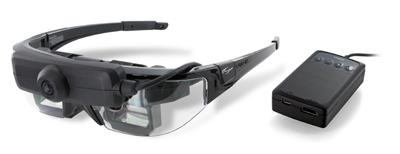
\includegraphics[width=0.4\textwidth]{vuzix}
  \caption{\ac{AR}-Brille \emph{Vuzix Star 1200}\ \cite{vuzix}}
  \label{fig:vuzix_star_1200}
\end{figure}

Für die Programmierung stehen die \ac{ICL}-Softwareumgebung des \ac{FZI}, sowie das \ac{ROS}-Framework \cite{ros} zur Verfügung.



\section{Headtracking}

Ziel des Headtrackings ist es, die Kopforientierung des Fahrers --~auch bei bewegtem Fahrzeug~--
%\todo{``fahrendem'' statt ``bewegendem''?}
% -> ich würde bei bewegt bleiben: es ist ja denkbar, dass das Auto nicht selber "fährt", aber trotzdem "bewegt" wird, beispielsweise auf einer Fähre oder so
sowohl relativ zum Fahrzeug als auch in Weltkoordinaten anzugeben. Unter Orientierung wird hier die Drehung entlang der X- (\emph{Roll}), Y- (\emph{Pitch}) und Z-Achse (\emph{Yaw}) verstanden:
\acs{RPY}.

Dazu wird die Inertialsensorik der \ac{AR}-Brille, bestehend aus zwei Gyroskopen, Beschleunigungssensor und Magnetometer, ausgewertet (Abs. \ref{headtracking_imu_subsec}).
Diese Daten werden mit einem geeigneten Filter-Algorithmus fusioniert (Abs.~\ref{headtracking_fusion_subsec}).
Die Kompensation der Eigenbewegung des Fahrzeugs wird in Abs. \ref{headtracking_marker_subsec} behandelt.

\subsection{Inertialsensoren}
\label{headtracking_imu_subsec}
Im folgenden Absatz werden die verschiedenen Sensoren vorgestellt. Dabei sei angemerkt, dass die gemessenen Daten in einem sogenannten \textit{Sensorkoordinatensystem $TF_{sensor}$} erfasst werden. Dieses ist um etwa $15^\circ$ in der Z-Achse rotiert zum \textit{Brillenkoordinatensystem $TF_{glasses}$}, welches seinen Ursprung in der Mitte des Brillenstegs hat. Dieses Koordinatensystem wurde so gewählt, dass es in etwa mit der Kameraposition der Brille übereinstimmt \footnote{Anbetracht der vorhandenen Messungenauigkeiten wurden die Translationen zwischen Sensor und Brillensteg sowie Kamera und Brillensteg vernachlässigt, da sie keinen eklatanten Einfluss auf die Orientierung der Brille bzw. des Kopfes haben.}. In Abb. \ref{fig:tf_baum_sensorik}

\todo[inline]{Ich bitte den Ersteller des TF-Baums sich dieser Grafik anzunehmen, der sieht sehr professionell aus, so was in abgespeckter Form brauchen wir hier auch, damit wir uns in den nachfolgenden Sections drauf beziehen können, bitte die Textreferenzen in \ref{headtracking_imu_subsec} dazu anpassen.}

\subsubsection{Gyroskop}
\label{headtracking_imu_gyro_subsubsec}

Die in der Brille enthaltenen Gyroskop unterschiedlicher Genauigkeit messen die Winkelgeschwindigkeiten $\omega$ in $[{\degree \over Sekunde}]$ bei Drehungen um die X-, Y- und Z-Achse. Durch
die Integration der Winkelgeschwindigkeiten über die Zeit kann die
Orientierung der Brille bestimmt werden.  

Die Rohdaten des Gyroskops sind fehlerbehaftet und enthalten einen
konstanten Fehleranteil, welcher \emph{Bias} bezeichnet wird. Somit wird
bei stationärer Brillenlage eine Geschwindigkeit $\omega \neq 0$
gemessen, welche in einem stationären Kalibriervorgang ermittelt werden
muss. Dazu werden die Sensordaten über einen kurzen Zeitraum bei
unbewegter Brille erfasst und über die Zeit gemittelt. Der so ermittelte
Wert wird von den Sensor-Rohdaten subtrahiert. Abb.  \ref{fig:gyro_bias}
zeigt die Daten vor und nach der Bias-Korrektur.

\begin{figure}[h]
   \centering
   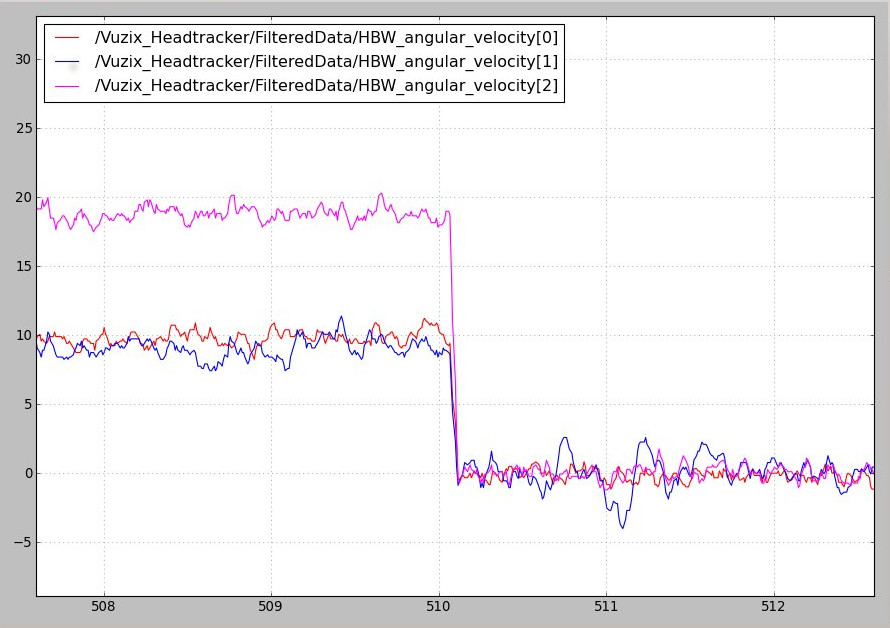
\includegraphics[width=0.45\textwidth]{stationary_calibration_before_after}
   \caption{Korrektur des Gyroskop-Bias}
   \label{fig:gyro_bias}
\end{figure}

Des Weiteren unterliegen die Sensordaten einem Rauschen. Daher wird als
nächster Schritt ein Tiefpassfilter verwendet, um dieses Rauschen zu
reduzieren. In unserem Fall hat sich ein Mittelwertfilter mit einer 
Fenstergröße von 5 als praktikabel erwiesen. Je höher die Fenstergröße gewählt wird,
desto stärker werden die Rohdaten geglättet, damit steigt jedoch auch
die Verzögerung der Daten. Abb. \ref{fig:lowpass-delay} zeigt den Effekt des Tiefpassfilters.

\begin{figure}[h]
   \centering
   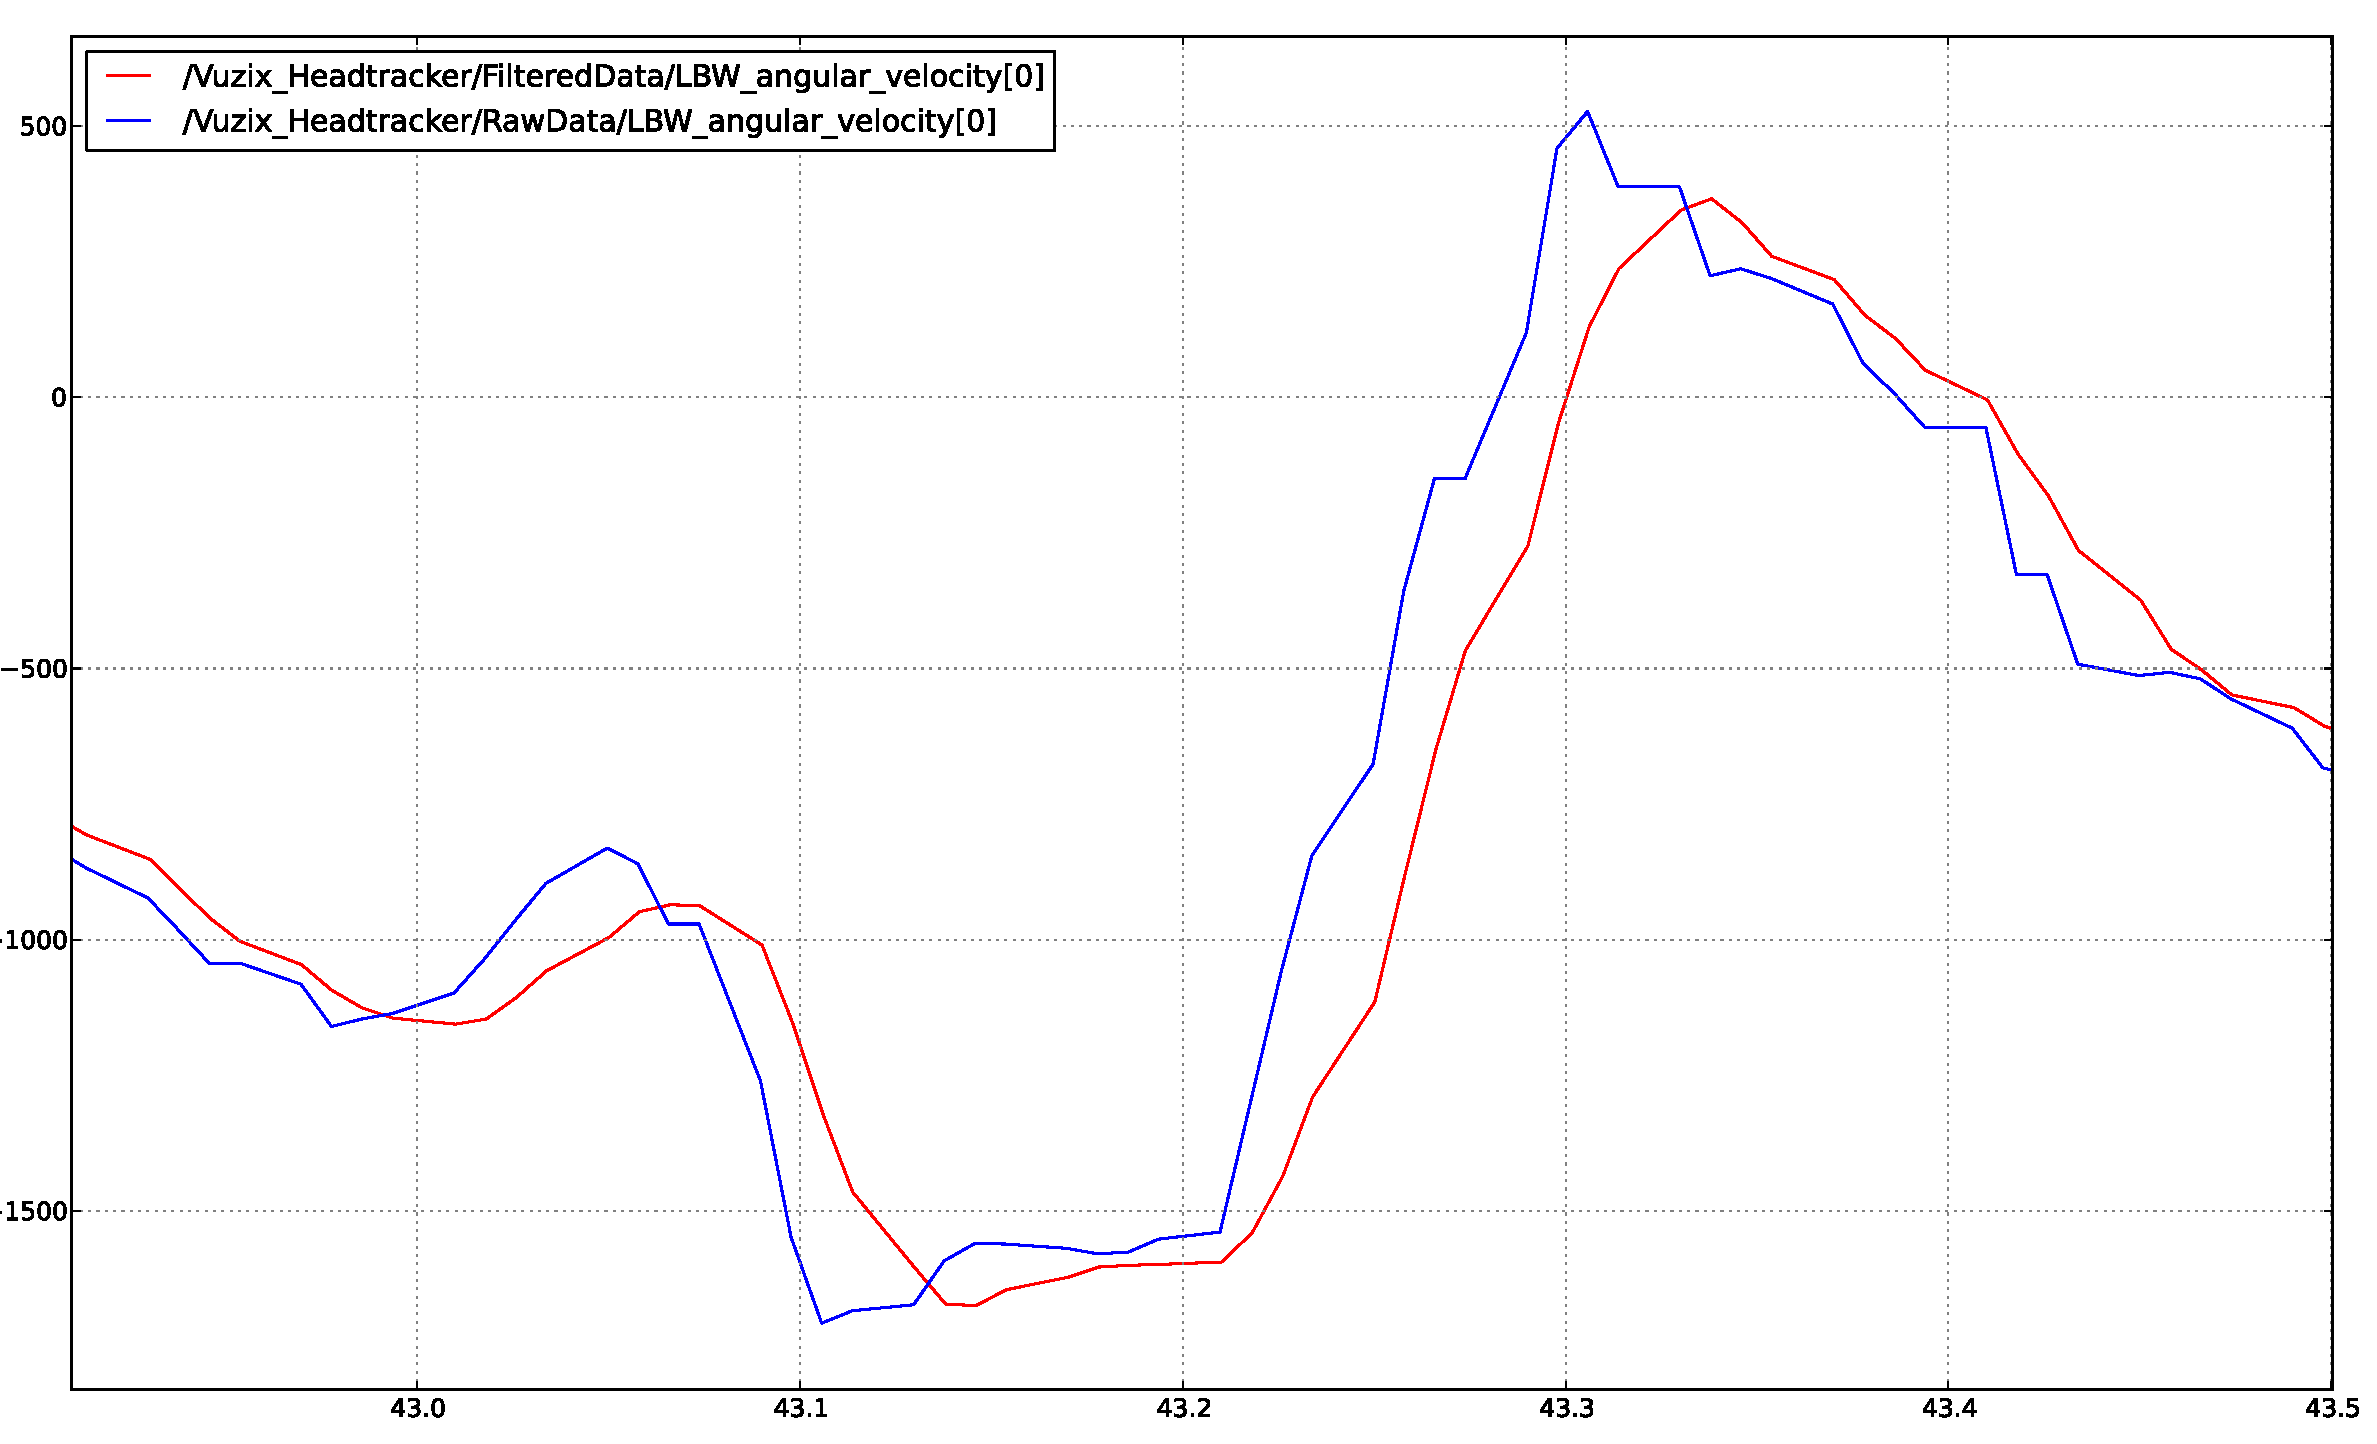
\includegraphics[width=0.45\textwidth]{FilteringDelay}
   \caption{Auswirkung des Tiefpassfilters: Ungefilterte Daten (blau) vs. gefilterte Daten (rot)}
   \label{fig:lowpass-delay}
\end{figure}

Die \ac{IMU} der Brille enthält zwei
Gyroskope, ein \emph{High Bandwidth} Gyroskop sowie ein
\emph{Low Bandwidth} Gyroskop. Die Gyroskope unterscheiden sich
hinsichtlich der Genauigkeit und des Wertebereiches. Das \ac{HBW}-Gyroskop
hat einen größeren Wertebereich, jedoch die geringere
Genauigkeit.

Die Wertebereiche der Gyroskope sind
in Tabelle \ref{tab:ranges-gyros} aufgeführt. Beide Gyroskope liefern
einen 12-Bit-Datenwert. Somit stellt ein Zählwert des \ac{LBW}-Gyroskops eine
kleinere Veränderung dar als beim \ac{HBW}-Gyroskop.
Dies bedeutet, dass das \ac{LBW}-Gyroskop eine höhere Genauigkeit besitzt.

\begin{table}[ht]
  \centering
  \begin{tabular}{ | c | c | c | }
    \hline
    & Min. & Max. \\ \hline
    \ac{LBW} & -420   & 420   \\ \hline
    \ac{HBW} & -1680   & 1680   \\
    \hline
  \end{tabular}
  \caption{Gyroskop-Wertebereiche in $[{\degree \over s}]$}
  \label{tab:ranges-gyros}
\end{table}


Zur Fusionierung des \ac{HBW}- und \ac{LBW}-Gyroskops kommt ein einfaches Schwellwertverfahren zum Einsatz. 
Im Wertebereich, welcher von beiden Gyroskopen abgedeckt wird, werden
die Sensordaten gemittelt. Wird der Wertebereich des \ac{LBW}-Gyroskops
überschritten, wird lediglich der Wert des \ac{HBW}-Gyroskops
zurückgeliefert.

\begin{equation}
    G = \left\{
    \begin{array}{ll}
        \frac{G_{HBW} + G_{LBW}}{2}, & G_{LBW} < G_{LBW_{max}}  \\
        G_{HBW}, & G_{LBW} = G_{LBW_{max}}
    \end{array}\right. \\
\end{equation}

\todo[inline]{Die Unterscheidung deckt nicht alle Fälle ab. Was ist mit dem größer-Fall?}

Aus den gefilterten Sensordaten wird daraufhin durch Integration über
die Zeit die Orientierung berechnet. Hierzu wird die Orientierung in einem Quaternion gespeichert, welches nach jeder Sensorabtastung aktualisiert wird. Hierbei ist $dt$ die Abtastrate der Gyroskop-Sensoren, welche 100Hz beträgt.

\begin{equation}
    \Delta q = quaternion({\omega_x \over dt}, {\omega_y \over dt}, {\omega_z \over dt}) \\
\end{equation}

\begin{equation}
    q_{t+1} = q_t * \Delta q
\end{equation}

Die durch das Gyroskop berechnete Orientierung reagiert schnell auf
Änderungen. Durch die Integration entsteht in jedem Integrationsschritt jedoch ein Fehler, welcher sich summiert. Dieser Fehler wird als \emph{Drift} bezeichnet. In den folgenden Abschnitten wird beschrieben wie Beschleunigungssensor und Magnetometer verwendet werden können, um diesen Fehler zu kompensieren.

% TR: Schöner Abschnitt  :-)


\subsubsection{Beschleunigungssensor}


Der Beschleunigungssensor misst die Beschleunigung entlang der X-, Y-
und Z-Achse, im Folgenden als $acc_x$, $acc_y$ und $acc_z$ bezeichnet.
Bei stationärer Brille wird lediglich die Erdbeschleunigung $\vec g$
gemessen, somit kann aus dem Beschleunigungsvektor die Orientierung der
Brille bezüglich der horizontalen Ebene bestimmt werden. Zu beachten
ist hierbei, dass durch eine Bewegung der Brille eine zusätzliche
Beschleunigung gemessen wird, welche die berechnete Orientierung
verfälscht. Dieser Fehler ist jedoch vernachlässigbar, da die berechnete
Orientierung lediglich zur Langzeitkorrektur verwendet wird.


Zur Verwendung des Beschleunigungssensors wird zunächst wie auch beim
Gyroskop ein Tiefpassfilter angewendet, um das Rauschen der Rohdaten zu
reduzieren.
Dabei wird ein Mittelwertfilter eingesetzt.
Als Fenstergröße wird die gleiche wie beim Gyroskop gewählt, da ein ungleicher Wert zu einer zeitlich inkonsistenten Datenfusion führen würde.

% XXX: die umrechung auf m/s2 hab ich mal rausgelassen, die ist ja glaub ich auch garnicht so wichtig und verwirrt den leser nur

Die Orientierung in Roll und Pitch kann direkt aus den Winkeln des Gravitationsvektors berechnet werden.

\begin{equation}
    roll = atan2(acc_y, acc_z)
\end{equation}

\begin{equation}
    pitch = -atan2(acc_x, \sqrt{ {acc_y}^2 + {acc_z}^2 })
\end{equation}

Die so bestimmten Roll- und Pitch-Werte sind frei von Drift, und können als Stützwerte für die aus den Gyroskopdaten berechneten Orientierungswerte verwendet werden.
Jedoch ist zu beachten, dass der Beschleunigungssensor nicht zuverlässig zur Berechnung des Yaw-Winkels verwendet werden kann.
Dies liegt darin begründet, dass sich die Sensordaten des Beschleunigungssensors nicht ändern, wenn sich der Sensor parallel zur Erdoberfläche befindet und um den Yaw-Winkel gedreht wird.


%  roll = atan2(acc_data[1], acc_data[2]);
%  pitch = -atan2(acc_data[0], sqrt(acc_data[1]*acc_data[1] + acc_data[2]*acc_data[2]));



\subsubsection{Magnetometer}
\label{headtracking_magnetometer_subsubsec}

Das Magnetometer wird im Rahmen des Praktikums zur Stützung des Yaw-Winkels (Drehung um die Z-Achse des Brillenkoordinatensystems $TF_{glasses}$) genutzt.\
Das verbaute Magnetometer misst in drei Achsen nach dem Funktionsprinzip der Wheatstoneschen Messbrücke \cite{renaudin2010complete} das Erdmagnetfeld.
Dieses Messverfahren führt zum einen zu einer kleinen und kostengünstigen Bauweise.
Zum anderen entstehen aber Messungenauigkeiten, die im Rahmen der Sensorkalibrierung beachtet und ausgeglichen werden müssen.

\begin{figure}[h]
   \centering
   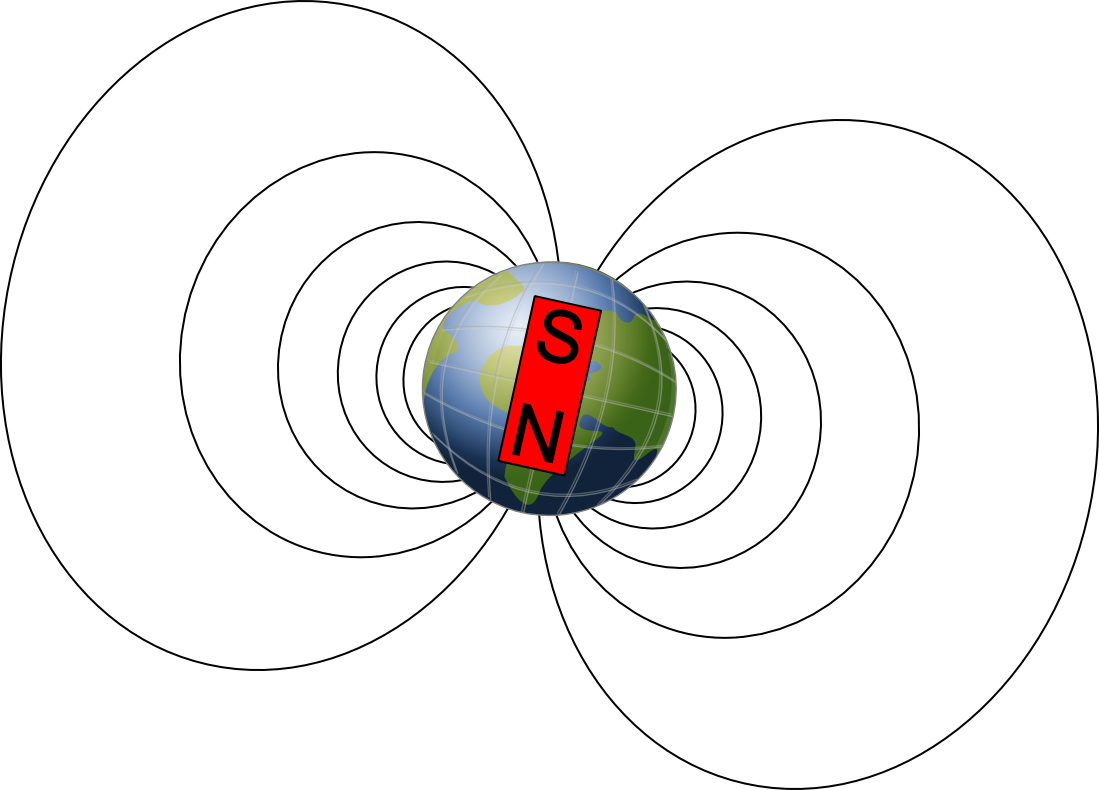
\includegraphics[width=0.4\textwidth]{earth-magnetic-field}
   \caption[mag_world]{Schematische Darstellung des Erdmagnetfelds \cite{mag_world_source}.}
   \label{fig:mag_world}
\end{figure}

\begin{figure}[h]
   \centering
   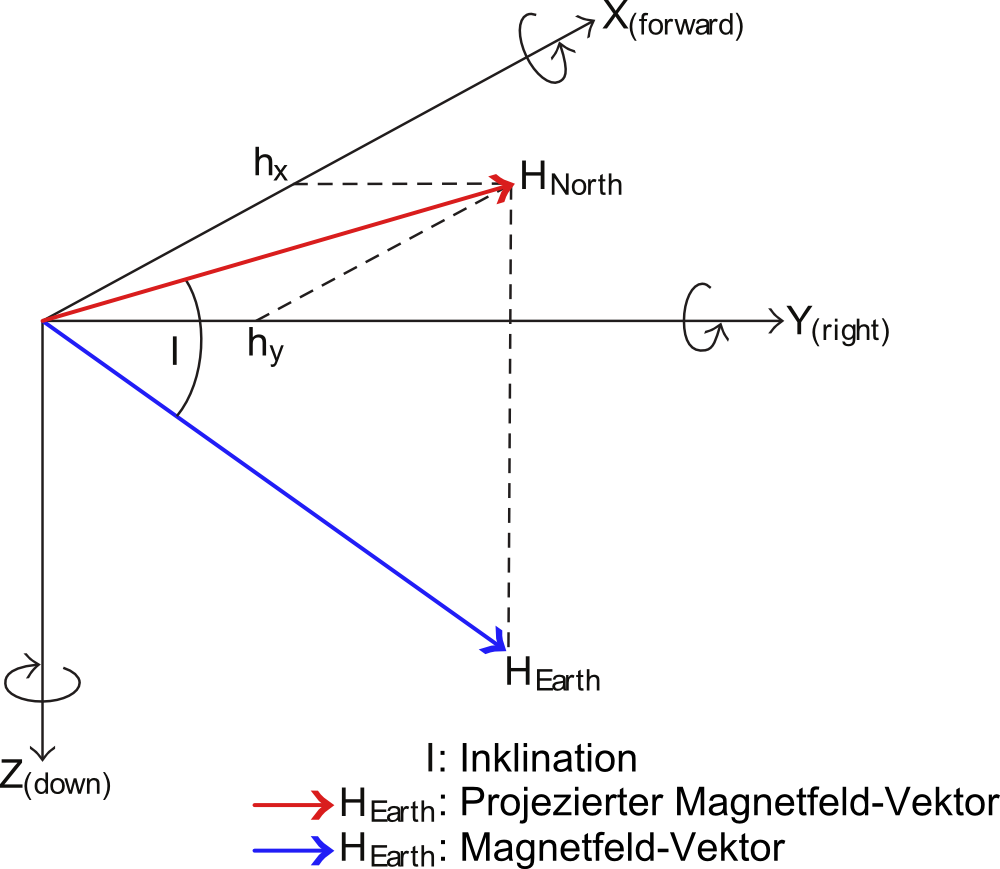
\includegraphics[width=0.4\textwidth]{magnetometer-yaw-calculation}
   \caption[mag_mapping]{Berechungsgrundlage des Magnetfeldvektors\cite{wang2006intelligent}}
   \label{fig:mag_mapping}
\end{figure}

Gemessen werden die Magnetfeldlinien der Erde, welche in Abb. \ref{fig:mag_world} dargestellt sind.
Diese sind abhängig von der aktuellen Position auf der Erdoberfläche\footnote{Tatsächlich verändert sich das Erdmagnetfeld auch über die Zeit hinweg.
Diese Änderung kann aber im Rahmen des Praktikums vernachlässigt werden, da es sich um eine sehr kleine Änderung handelt (\zB für den Praktikumsort Karlsruhe ca. $1^\circ 46$'~$7.8$ arcmin/Jahr im Deklinationswinkel).}.
Sobald das Erdmagnetfeld nicht am Äquator gemessen wird, wie beispielsweise in Karlsruhe der Fall bei ca. $49^\circ$ geographischer Breite, muss der Inklinationswinkel\footnote{Bezeichnet den Neigungswinkel des örtlichen Erdmagnetfeldes zur Horizontalen.} bei der Messung mit beachtet werden.
Dieser wird in Abb. \ref{fig:mag_mapping} mit I beschrieben.
Die Abbildung \todo{@honnel: Vorschlag: Die Abbildung von den 3D-Magentometerwerten auf die XY-Ebene ...} auf die XY-Ebene wird durch folgende Formel bewerkstelligt:

\begin{equation}
    \varphi = atan2(h_y,h_x)
\end{equation}

Dabei sind $h_x$ und $h_y$ die Anteile des Magnetfeldvektors $H_{Earth}$ in X- sowie Y-Richtung.

Der gemessene 3D-Magnetfeldvektor ist zunächst unkalibriert und einheitenlos.
Daher ist zuerst eine Kalibrierung der gemessenen Werte notwendig, um sie weiterverarbeiten zu können.
Diese Kalibrierung hat zum Ziel, einen kanalspezifischen Bias auszugleichen. 
Dieser entsteht durch die bereits angesprochenen Messungenauigkeiten des Sensors sowie durch sogenannte \textit{Hard Iron} Störeffekte, welche durch eigenständige Magnetquellen induziert werden.
Beispiele für diese Störeffekte sowie die letztlich kalibrierten Daten sind in Abb. \ref{fig:mag_kugel_plots} als Kugelplots dargestellt.

\begin{figure}[ht]
\centering
\subfigure[Unkalibrierte Magnetometerdaten mit Hard Iron Störeinflüssen]{
    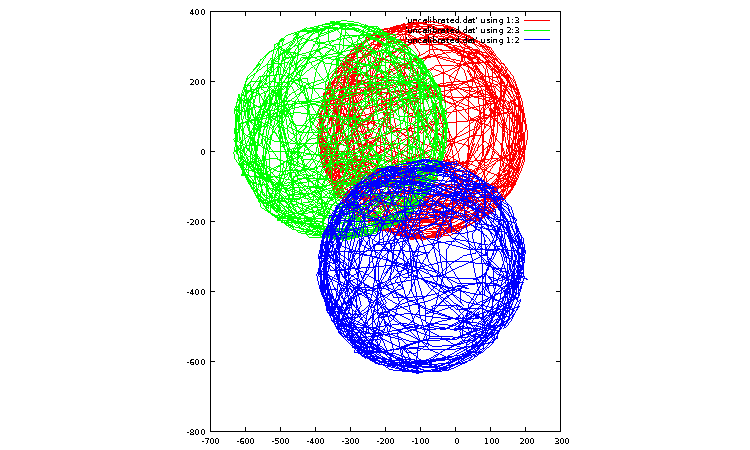
\includegraphics[width=0.5\textwidth]{uncalibrated}
    \label{fig:subfig1}
}
\subfigure[Kalibrierte Magnetometerdaten]{
    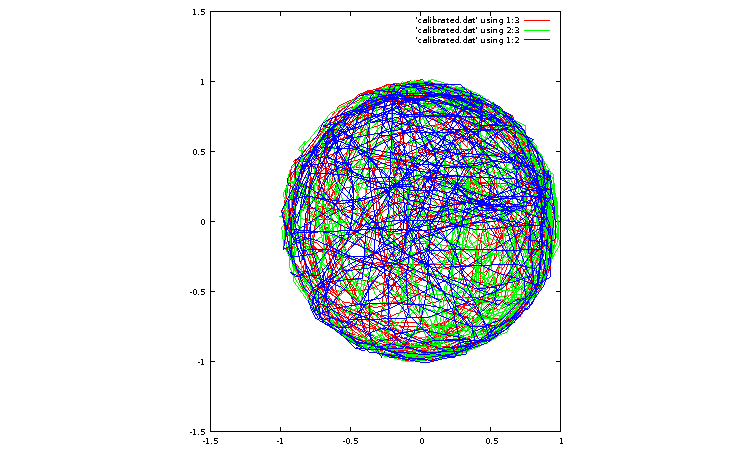
\includegraphics[width=0.5\textwidth]{calibrated}
    \label{fig:subfig2}
}

\caption[]{2D-Sichten auf Kugel aus Magnetometerdaten}
\label{fig:mag_kugel_plots}
\end{figure}

Im Gegensatz zu den bisher vorgestellten Sensoren wird die Kalibrierung des Magnetometers durch Bewegung durchgeführt.
Ziel ist es, die Wertebereiche in allen drei Achsen zu erfassen.
Dafür wird die Brille in allen Achsen um mindestens $360^\circ$ gedreht, um die minimalen und maximalen Werte zu registrieren. 
Des Weiteren werden die Daten noch durch einen Tiefpassfilter geglättet, sowie auf einen Wertebereich von $[-1,1]$ abgebildet.
Der Tiefpassfilter wird wie in Abs. \ref{headtracking_imu_gyro_subsubsec} bereits beschrieben durchgeführt. 
Die Anwendung der Kalibrierung und Normierung wird durch nachfolgende Formel bewerkstelligt:
\begin{equation}
    m_{norm} = \frac{m_{raw}- \frac{m_{\delta}}{2}}{2~m_{\delta}},  {\delta}~=~m_{max}~-~m_{min}
\end{equation}
Dabei bezeichnet $m_{norm}$ einen normierten Magnetfeldvektorkanal, $m_{raw}$ die Rohdaten des jeweiligen Kanals und $m_{\lbrace max, min\rbrace}$ den gemessenen Maximal- bzw. Minimalwert.

Ursprünglich war die Verwendung des Magnetometers zur Stützung des Yaw-Winkels fraglich, da der Einsatz im Versuchsträger \emph{CoCar} viele magnetische Störquellen in Form der vorhandenen Boardtechnik vermuten lies. 
Allerdings konnten durch mehrere Testläufe im Fahrzeug keine größeren Störeffekte gemessen werden. Trotz allem muss eine Kalibrierung in einem möglichst störfreien Umfeld durchgeführt werden, da durch Störquellen (wie bspw. ein Dauermagnet, eine Tastatur, \oae) die Messdaten wie in Abb. \ref{fig:uncalibrated_error} zu erkennen wesentlich beeinflusst werden. In Abb.~\ref{fig:uncalibrated_error} sind unkalibriete Messdaten dargestellt (Kreise liegen nicht über einander). Die Störungen sind dadurch zu erkennen, dass sie außerhalb der Kreise der einzelnen Kanäle liegen.

\begin{figure}[ht]
	\centering
    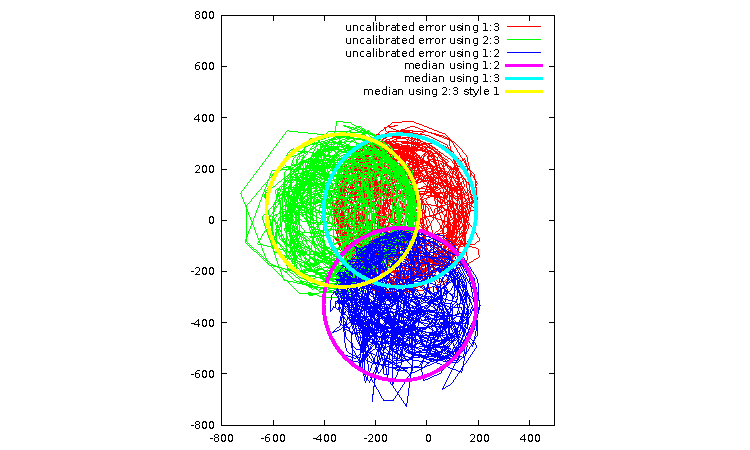
\includegraphics[width=0.5\textwidth]{uncalibrated_error}
	\caption[]{2D-Sichten auf Kugel aus Magnetometerdaten mit Störquelle}
	\label{fig:uncalibrated_error}
\end{figure}

Um die Magnetometerdaten letztlich zur Stützung des Yaw-Winkels zu nutzen, werden die Daten zuerst in das Weltkoordinatensystem transformiert.
\todo{Es geht nicht hervor welche Daten hier gemeint sind: Nur Mag oder auch Gyro, Acc? Hat das auch wieder mit der 15-Grad-Verdrehung zu tun? Haben die Implementierung leider grad nicht hier zum Nachschauen ;)}
Danach wird das vorhandene Rotationsquaternion $q_{gyro,acc}$ mit $q_{mag}$ (Magnetometer-Quaternion) interpoliert.
Das genaue Verfahren wird im nachfolgenden Abs.~\ref{headtracking_fusion_subsec} vorgestellt.


\subsection{Sensordaten-Fusion}
\label{headtracking_fusion_subsec}
Die Sensordaten-Fusion beschreibt die Verknüpfung von mehreren Sensoren um Informationen besserer Qualität zu gewinnen. In diesem Projekt gilt des die aufbereiteten Daten aus beiden Gyroskopen, Beschleunigungsensor und Magenetometer derart zu fusionieren, dass letztlich die zu ermittelnde \emph{Orientierung} des Kopfes möglichst exakt bestimmt werden kann. Da die bereits vorgestellten Sensoren jeweils eigene Vor- und Nachteile hat müssen diese bestmöglich ausgenutzt werden. In den folgenden Abschnitten werden unterschiedliche Fusionsansätze dargestellt und entsprechend der Aufgabenstellung des Projekts bewertet. 

\subsubsection{Madgwick-Filter}
Die Filterung nach Madgwick \cite{madgwick2010efficient} gilt als neuartiger Ansatz zur Bestimmung der Orientierung basierend auf Gyroskop, Beschleunigungssensor und Magnetometer.
Es wird dabei versucht die magnetische Distorsion sowie der Bias-Trift des Gyroskopes auszugleichen.
Berechnungsgrundlage ist dafür eine auf Quaternionen-basierte Darstellungsform, welche in einem Gradienten-Abstiegsverfahren zum Einsatz kommt.
Vorteile dieses Ansatzes sind seine niedrigen Berechnungskosten, Effektivität bei niedrigen Sampleraten und ein hoher Grad an Parametrisierung der eine Anpassung an die jeweiligen Sensor- und Umgebungscharakteristiken zulässt.

Auch wenn der Madgwick-Filter bereits als fertige ROS-Node\footnote{\url{http://wiki.ros.org/imu_filter_madgwick}} vorhanden ist und bessere Ergebnisse als der Kalman-Filter liefern soll, haben wir uns gegen den Madgwick-Filter entschieden, da unsere bestehende Implementierung nur schwer an den Madgwick-Filter angepasst werden konnte und dadurch der erzielte Mehrwert so nur schwer nachvollziehbar bzw. debuggbar gewesen ist. 


\subsubsection{Kalman-Filter}
Beim Kalman-Filter Verfahren \todo{cite} handelt es sich um eine probabilitische Methode der Zustandsschätzung.
Dabei fließen in einem ersten \emph{Prädiktionsschritt} vorhergemachte Annahmen inklusive dazugehöriger Fehlerwahrscheinlichkeiten in die Berechnung ein.
Danach wird in einem zweiten Schritt, der \emph{Innovationsschritt}, eine Beobachtung mit dazugehöriger Messungenauigkeit mit einbezogen.

Um bei einer fehlerbehafteten Beobachtung den Systemzustand zu korrigieren, müssen diese Beobachtungen über mathematische Gleichungen beschreibbar und Fehlerverteilungen für Sensoren bekannt sein. Diese Informationen sind uns während der Bearbeitung des Projekts nicht bekannt gewesen.
Infolgedessen konnte eine Modellierung gemäß dem Kalman-Filters nicht durchgeführt werden. 
Des weiteren war unklar ob durch eine solche Umsetzung tatsächliche Vorteile erzielt werden können, da die Änderung eines plötzlichen Ereignis (Kurvenfahrt) über mehre Zeitschritte hinweg angepasst wird und somit eine mögliche Latenz hinzugefügt werden könnte.

\subsubsection{Komplementär-Filter}
Nach Brooks und Iyengar \cite{Brooks.1998} hat eine komplementäre Fusion das Ziel, die Genauigkeit von Daten zu verbessern. 
Dabei wirken die Sensoren unabhängig voneinander und liefern unterschiedliche Erkenntnisse und Sichtbereiche, die die Orientierung zu unterschiedlichen Zeiten verbessert.

Die Gyroskope sind wie bereits erwähnt bei einer langen Laufzeiten fehleranfällig und erzeugen einen Drift. 
Daher wird im ersten Schritt eine SLERP-Interpolation (Sperical Linear Interpolation) eingesetzt, die bei jedem Zeitschritt die Orientierung der Gyroskope zu $95\%$ und Orientierung des Beschleunigungssensor zu $5\%$ berücksichtigt. Hierbei wird das \emph{roll} und \emph{pitch} gestützt. Der zweite Schritt zielt auf die Verbesserung von \emph{yaw} ab. Eine weitere Interpolation verrechnet dieses Ergebnis mit den aufbereiteten Magnetometerwerten zu $5\%$ pro Zeitschritt. Formal lässt sich die Gewichtung folgendermaßen beschreiben:
\begin{equation}
    gyro.slerp(0.05, acc).slerp(0.05, mag)
\end{equation}
\todo{Formel in mathematische Formel umbauen, nicht Quellcode}

Eine Übersicht der Fusionierung mit dem Komplementär-Filter ist Abbildung \ref{fig:fusion_complementary} zu entnehmen.

\begin{figure}[ht]
	\begin{center}
		\scalebox{0.77}{
	\begin{tikzpicture}[%
		>=stealth, % Aussehen der Pfeilspitzen
		->, % Linien als Verbindungslinien
		looseness=.7, % Kr"ummung der Pfeile mit Option ’bent’
		auto, % Position des Ankers f"ur Node Labels
		color=black, % Farbe aller Linien
		%text=red, % Textfarbe in den Matrix-Nodes
		line width=1pt, % Linienst"arke f"ur alle Elemente
		text centered
	]
		\tikzstyle{every node}=[shape=rectangle,draw,fill=white,
		anchor=center] % Stil der Node-Beschriftung der
	\node[rectangle, rotate=-30, draw=orange, text width=2.5cm, outer sep=3pt, minimum size=1.5cm] at (0.6,4.5) {\textbf{$\alpha X+(1-\alpha)Y$}};
	\node[rectangle, font=\bfseries, double=green, text width=2.0cm, outer sep=3pt, minimum size=1.5cm](gyro) at (-7.0,5.5) {Gyro};
	\node[rectangle, font=\bfseries, double=green, text width=2.0cm, outer sep=3pt, minimum size=1.5cm](acc) at (-3.0,5.5) {Acc};
	
	\node[rectangle, font=\small, text width=2.5cm, outer sep=3pt, minimum size=1.5cm](interpol1) at (-3.0,2.5) {Interpolation \\ \textit{(SLERP)}};
	
	\node[rectangle, font=\small, text width=2.5cm, outer sep=3pt, minimum size=1.5cm](interpol2) at (-3.0,-2.5) {Interpolation \\ \textit{(SLERP)}};
	\node[rectangle, font=\bfseries, double=green, text width=2.0cm, outer sep=3pt, minimum size=1.5cm](mag) at (-7.0,-2.5) {Mag};
	
	\node[draw=none] at (-0.5, 0.5)(imageAbove) {\scalebox{0.33}{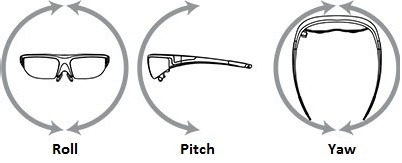
\includegraphics{rpy}}};
	\node[draw=none] at (-1.7, -0.5) {\scalebox{0.02}{
\includegraphics{Yes}}};
	\node[draw=none] at (-0.5, -0.5) {\scalebox{0.02}{
\includegraphics{Yes}}};
	\node[draw=none] at (0.75, -0.5) {\scalebox{0.02}{
\includegraphics{cross}}};
	
	\node[draw=none] at (1.0, -2.5)(imageBelow) {\scalebox{0.33}{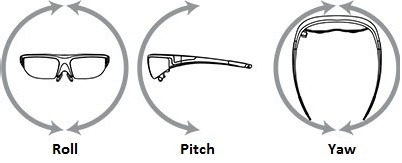
\includegraphics{rpy}}};
	\node[draw=none] at (-0.2, -3.5) {\scalebox{0.02}{
\includegraphics{Yes}}};
	\node[draw=none] at (1., -3.5) {\scalebox{0.02}{
\includegraphics{Yes}}};
	\node[draw=none] at (2.2, -3.5) {\scalebox{0.02}{
\includegraphics{Yes}}};

	\draw[orange, line width=2] (gyro) to[out=-90,in=-180] node[black, above, draw=none, fill=white, font=\small]{$0.95$} (interpol1);
	\draw[orange, line width=2] (acc) -- node[black, above, draw=none, fill=white, font=\small]{$0.05$} (interpol1);
	\draw[orange, line width=2] (interpol1) -- node[black, above, draw=none, fill=white, font=\small]{$0.95$} (interpol2);
	\draw[orange, line width=2] (mag) -- node[black, above, draw=none, fill=white, font=\small]{$0.05$} (interpol2);
	\draw[orange, line width=2] (interpol2) -- (imageBelow);
	
	\end{tikzpicture}}
	\end{center}
   \caption[]{Fusion -- Komplementärfilter}
   \label{fig:fusion_complementary}
\end{figure}

\subsection{Kompensation Störgröße Fahrzeug}
\label{headtracking_marker_subsec}

Bei einem stationären Fahrzeug genügt es, die Kopforientierung mittels \acs{IMU}-Daten der Brille zu bestimmen.
Die gesuchte Kopforientierung relativ zum Fahrzeug stimmt dabei mit der Kopforientierung bezüglich der Weltkoordinaten überein.
Sobald sich das Fahrzeug jedoch bewegt, wird die Schätzung der Kopforientierung verfälscht.
Fährt das Fahrzeug beispielsweise eine Kurve, so wird die von der IMU gemessene Drehung als Änderung des Yaw-Winkels der Kopforientierung interpretiert, obwohl der Fahrer in Bezug zum Fahrzeug weiterhin geradeaus blickt.

Eine weitere Störquelle stellt die Fahrzeugelektronik und die damit einhergehenden Änderungen des Magnetfelds dar.
Diese Störungen wirken sich negativ auf das zur Driftkorrektur eingesetzte Magnetometer aus (siehe Abschnitt \ref{headtracking_magnetometer_subsubsec}).

Zur Korrektur der Fehlschätzung aufgrund der genannten Einflüsse werden zwei Ansätze untersucht, die die Bestimmung der Kopforientierung relativ zum Fahrzeug stützen.
Abb.~\ref{fig:tracking_ansaetze} zeigt die beiden Ansätze konzeptionell.

\begin{figure}[h]
  \centering
  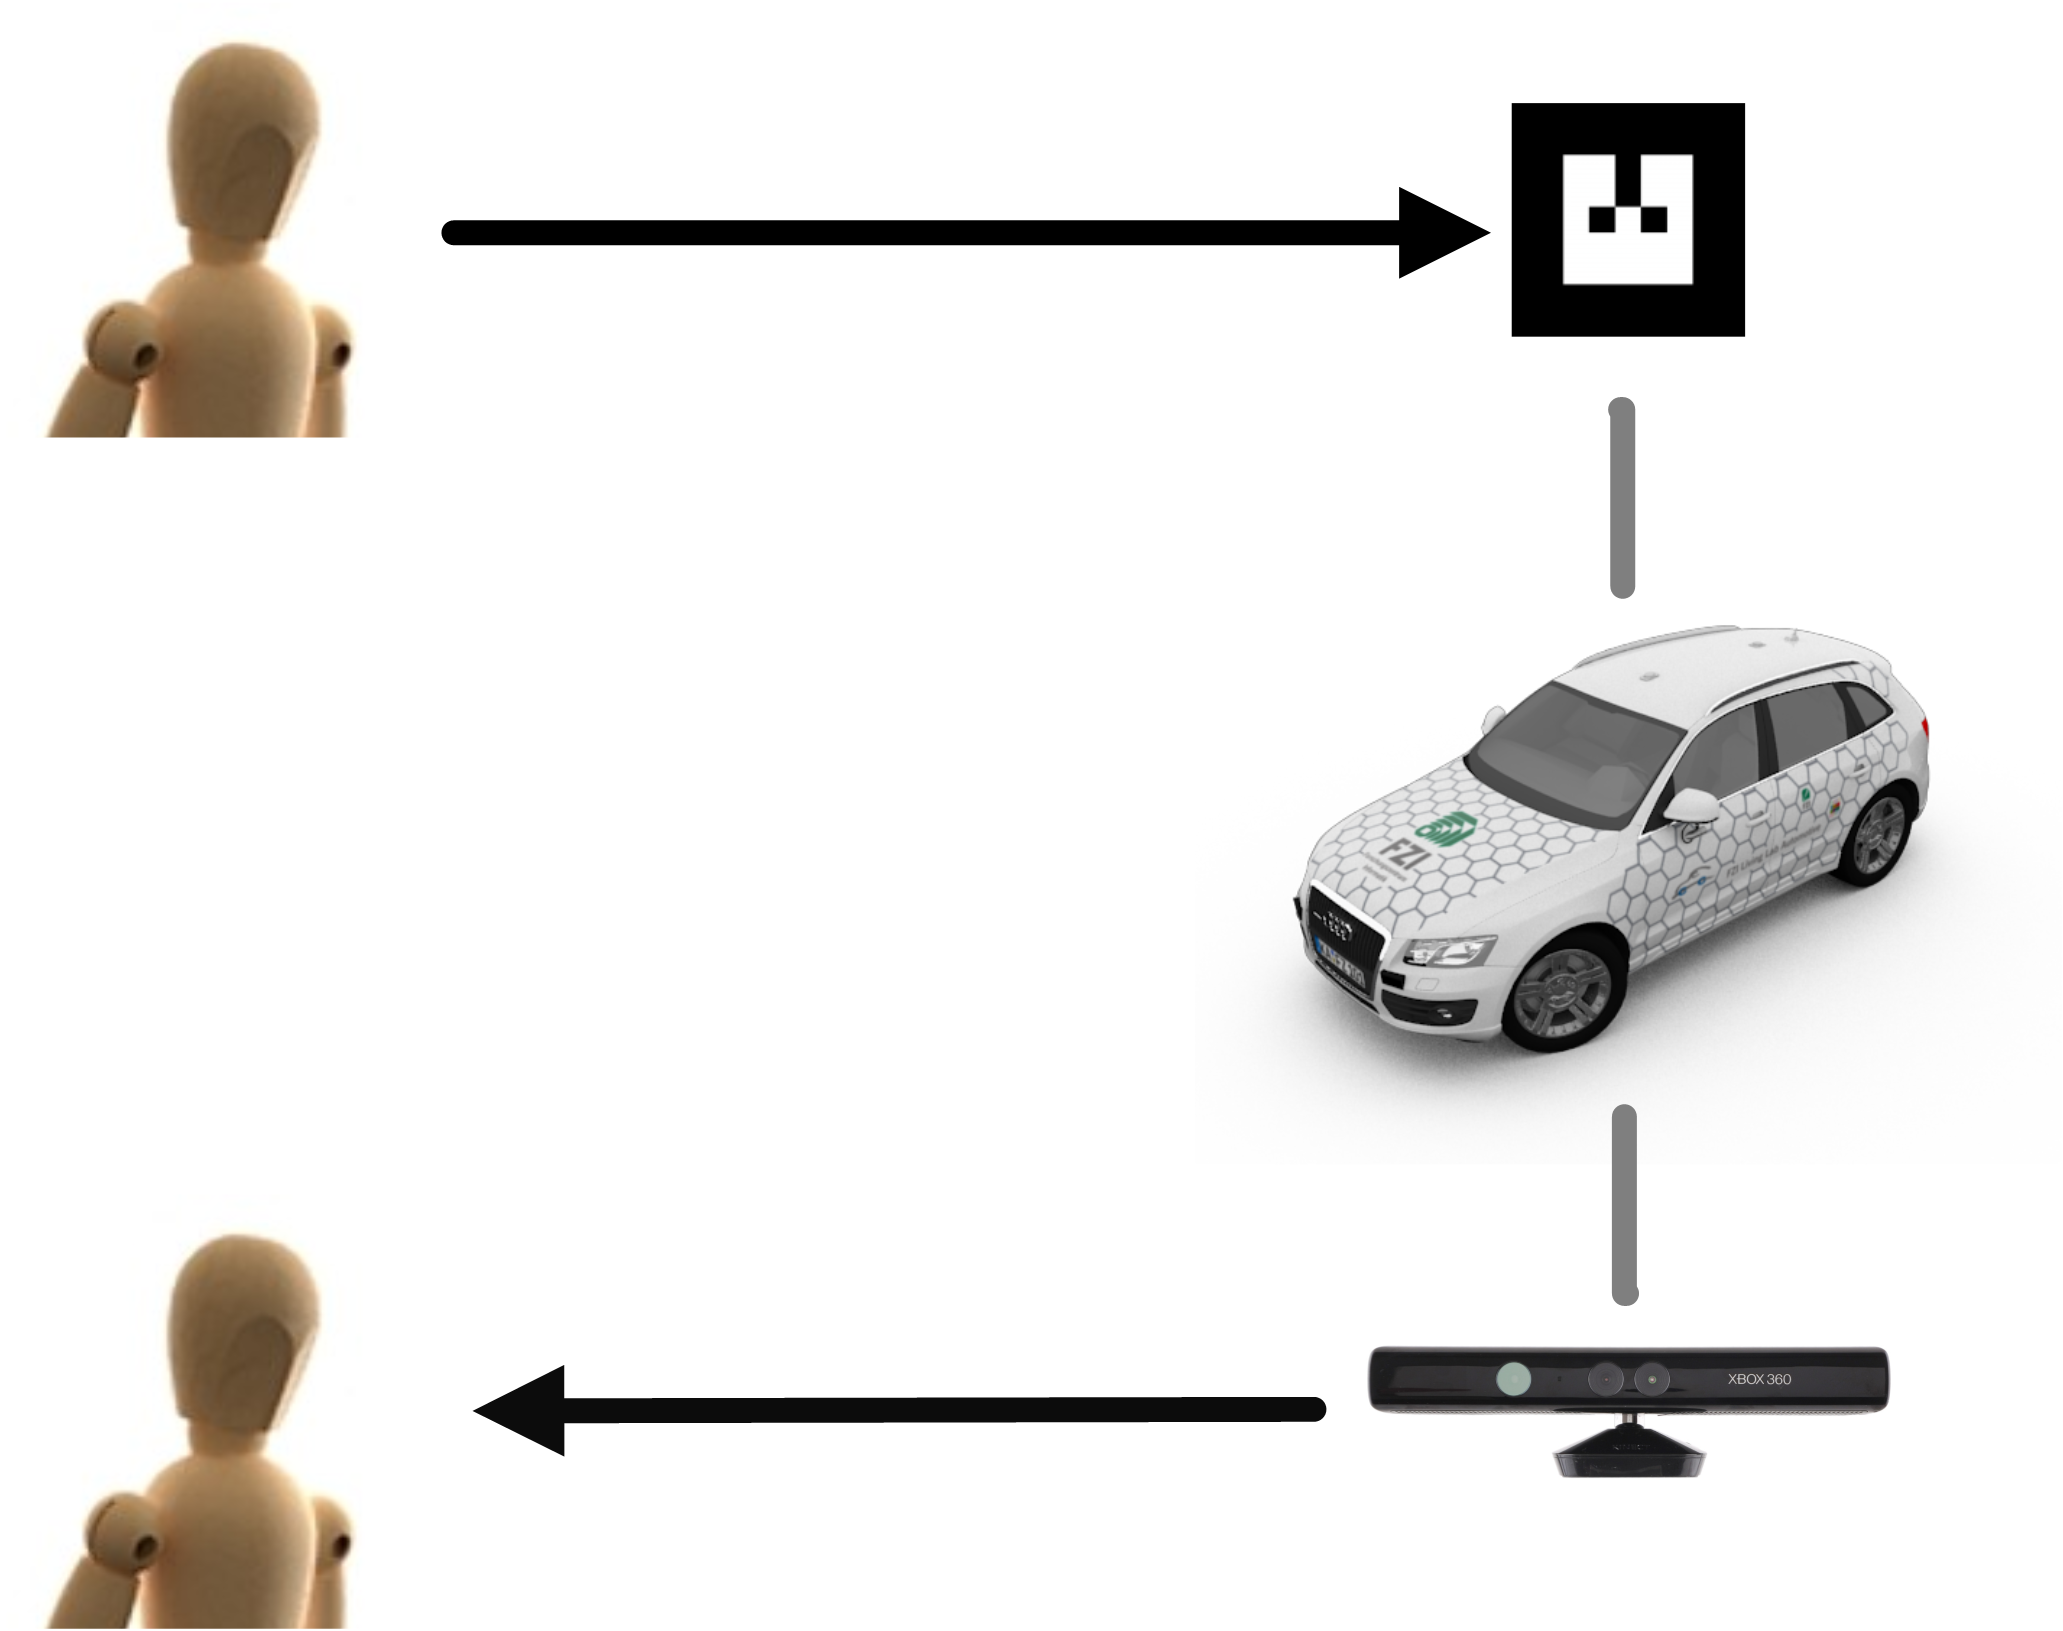
\includegraphics[width=0.4\textwidth]{Tracking_Ansaetze}
  \caption{Tracking-Ansätze: unten: Face-Tracking mit stationärer Kamera und bewegtem Kopf; oben: Marker-Tracking mit stationärem Marker und beweglicher Kamera }
  \label{fig:tracking_ansaetze}
\end{figure}


\subsubsection{Ansatz: Face-Tracking}
\label{headtracking_facetracking_subsubsec}

Die Idee beim Face-Tracking-Ansatz ist es, zu untersuchen, inwieweit die bestehende Hardware- und Software-Umgebung des CoCars für die Bestimmung der Kopforientierung verwendet werden kann.
Das Fahrzeug verfügt über eine fest installierte Kinect-Kamera, die auf den Fahrer ausgerichtet ist.
Für diese Kamera wurde am \ac{FZI} bereits ein Algorithmus zur Blickrichtungserkennung des Fahrers implementiert.
Der Algorithmus benutzt dafür ein Gesichtsmodell.
Das Gesichtsmodell berücksichtigt jedoch keine Brille.
Trägt der Fahrer eine Durchsichtbrille, ist ein Teil des Gesichts verdeckt.
Hierdurch wird die Erkennungsleistung stark beeinträchtigt.
Ein möglicher Ausweg ist das Einlernen des Gesichtsmodells mit Brille.
Jedoch ist die Spiegelung der von der Kinect verwendeten Infrarot-Strahlung an der Brille weiterhin problematisch.
Der Ansatz wird aus einem weiteren Grund nicht weiter verfolgt:
Die Verwendung von zusätzlicher Hardware schränkt die Wiederverwendbarkeit des Algorithmus zur Bestimmung der Kopforientierung ein.
Stattdessen fällt die Entscheidung auf einen Marker-Tracking-Ansatz, der alleine mit der Brillen-Hardware auskommt.


\subsubsection{Ansatz: Marker-Tracking}
\label{headtracking_markertracking_subsubsec}

Beim markerbasierten Tracking handelt es sich um ein optisches Trackingverfahren.
Dabei wird die Position und Orientierung eines speziellen Markers bestimmt, der im Kamerabild zu sehen ist.
Das Tracking übernimmt das \ac{ROS}-Paket \emph{ar\_track\_alvar}~\cite{ros_ar_track_alvar}, ein Wrapper für die Bibliothek \alvar.
Mit \alvar \ lassen sich Marker generieren, identifizieren sowie deren Posen im Kamerabild bestimmen - vorausgesetzt es wird eine kalibrierte Kamera verwendet.
Die Kamerakalibrierung kann mit dem \ac{ROS}-Paket \emph{camera\_calibration}~\cite{ros_camera_calibration} unter Verwendung eines Kalibrierschachbretts durchgeführt werden.
\alvar \ ermittelt die Pose des Markers in Bezug zum Kamerakoordinatensystem.
Für die Anwendung ist jedoch die Orientierung der Kamera von Interesse.
Sie wird als Kopforientierung interpretiert.
Wird der Marker als stationär angenommen, so kann die Inverse der von \alvar \ bestimmten Markerpose als Kamera- und somit als Kopfpose aufgefasst werden.
Abb.~\ref{fig:marker_in_vehicle_driver_view} zeigt den im Versuchsfahrzeug angebrachten Marker aus der Perspektive eines Fahrers.

\begin{figure}
  \centering
  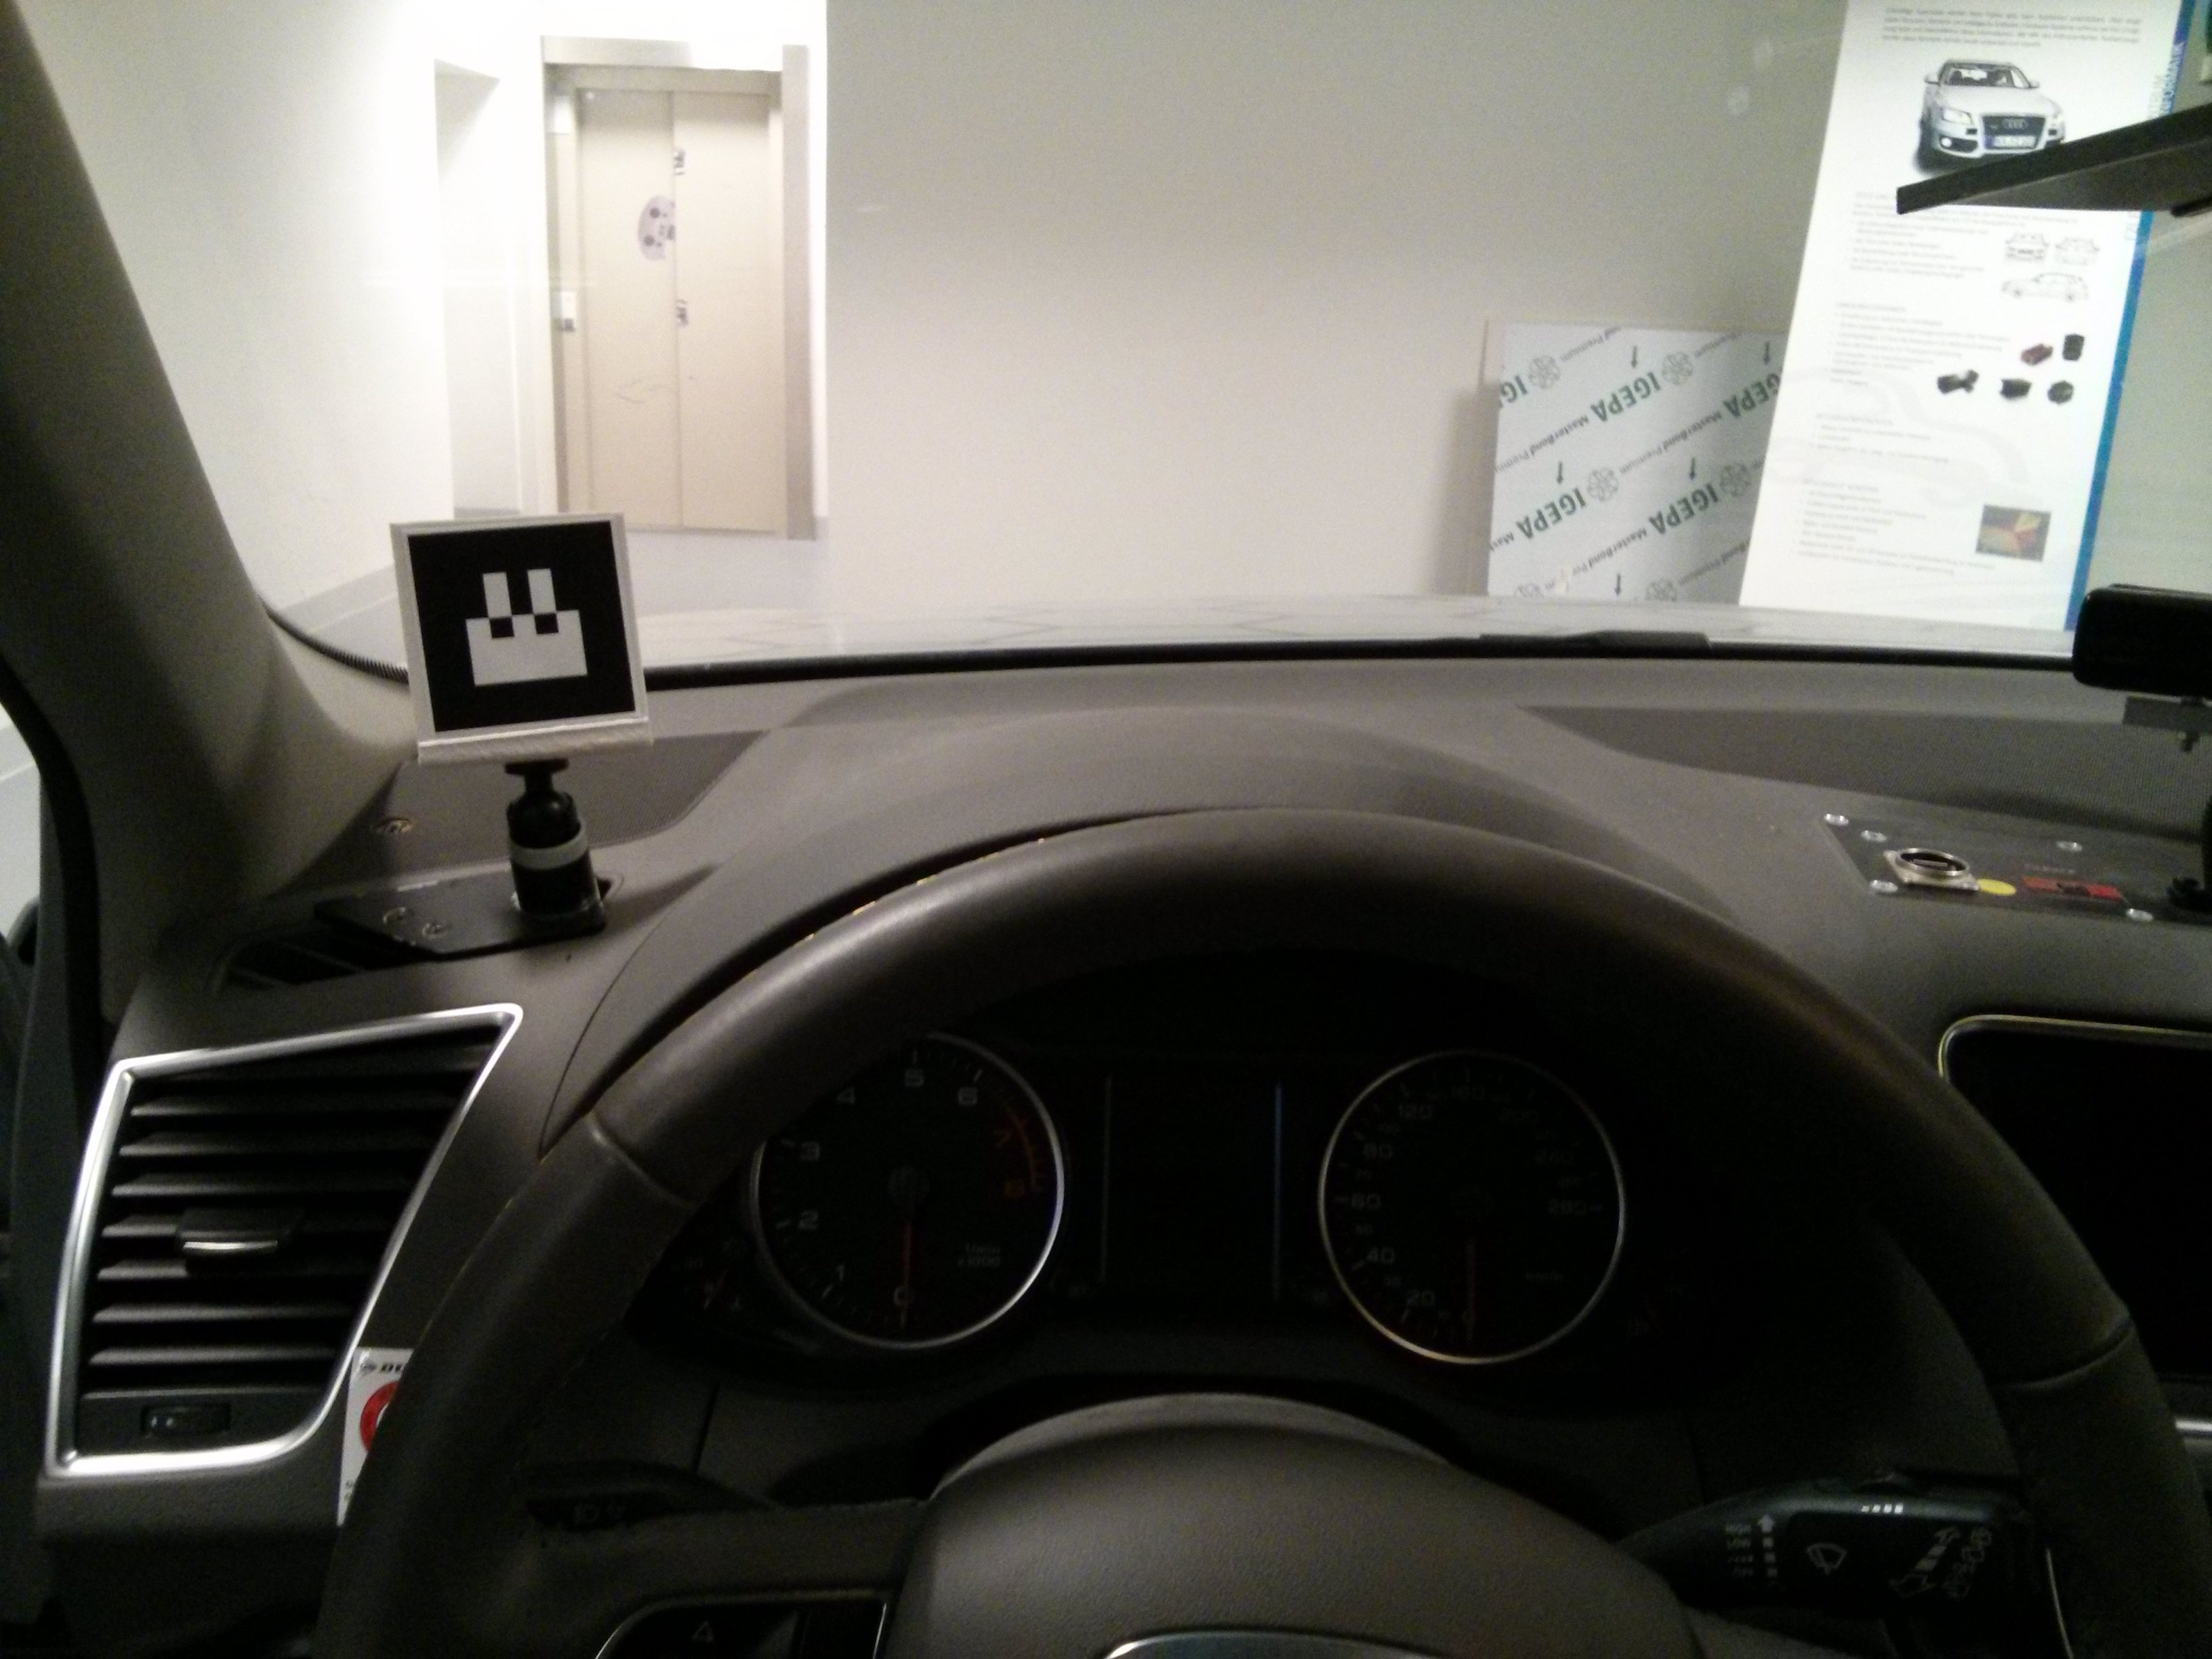
\includegraphics[width=0.4\textwidth]{marker_in_vehicle}
  \caption{Marker im Fahrzeug aus Fahrerperspektive.}
  \label{fig:marker_in_vehicle_driver_view}
\end{figure}

\begin{figure}
  \centering
  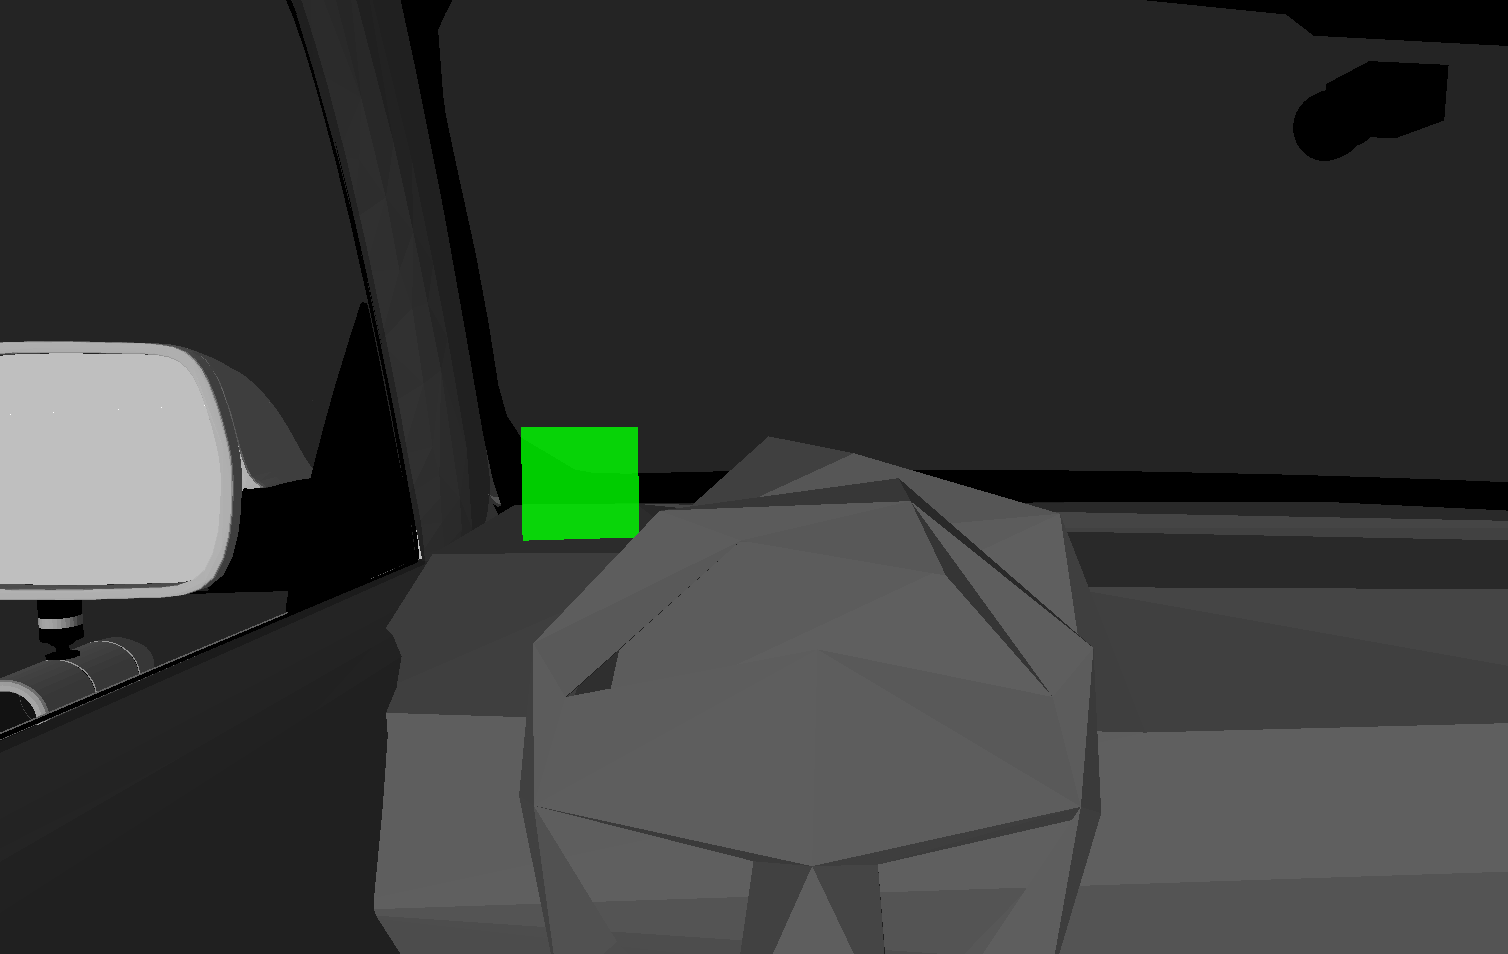
\includegraphics[width=0.4\textwidth]{Fahrerperspektive_ohne_Brille_RVIZ}
  \caption{Marker im Fahrzeug-Modell aus Fahrerperspektive.}
  \label{fig:marker_in_vehicle_model_driver_view}
\end{figure}

Damit die berechnete Orientierung des Kopfes in Bezug zum Fahrzeug steht, muss der Marker im Fahrzeug kalibriert werden.
Die Kalibrierungsdaten setzen sich aus Position und Orientierung des Markers angegeben in Fahrzeugkoordinaten zusammen.
Für die Kalibrierung des Markers im Fahrzeug stehen drei Varianten zur Wahl:
\begin{enumerate}
 \item Manuelle Ausmessung im Versuchsfahrzeug.
 \item Schätzung anhand der durch \alvar \ ermittelten Markerpose.
 \item Schätzung anhand des 3D-Fahrzeugmodells.
\end{enumerate}

Mit der ersten Variante lassen sich die Kalibrierungsdaten am genauesten bestimmen.
Allerdings ist der Aufwand für die Ermittlung auch am größten.
Die erste Variante hat mit der zweiten Variante gemein, dass sie anfällig für Variationen der Markerpose im Fahrzeug sind. Wird der Marker beispielsweise aus- und wieder eingebaut, ist es schwierig, den Marker in die zuvor kalibrierte Pose zu bringen.
Folglich muss die Kalibrierung neu durchgeführt werden.
Die dritte Variante ist mit dem geringsten Zeitaufwand verbunden und bietet gleichzeitig die größte Flexibilität.
Das zur Verfügung stehende Fahrzeugmodell ist dabei auch hinreichend genau.
Mittels \emph{dynamic\_reconfigure}-Paket~\cite{ros_dynamic_reconfigure} kann eine grafische Benutzerschnittstelle zur Konfiguration der Posenparameter des Markermodells generiert werden.
So lassen sich die Parameter auch zur Laufzeit anpassen.
Unter Nutzung der rviz-Ansicht kann die konfigurierte Markerpose visuell überprüft werden (siehe Abb.~\ref{fig:marker_in_vehicle_model_driver_view}).

Die Positionsangabe der von \alvar\ berechneten Markerpose wird in der Anwendung nicht genutzt, da die Kopfposition des Fahrers zur Vereinfachung als statisch angenommen wird.
Lediglich die Orientierung fließt in die folgende Fusion ein.

\subsubsection{Fusion IMU- und Kameraorientierung}
\label{headtracking_markerfusion_subsubsec}

Ziel der Fusion der mittels IMU-Daten berechneten Orientierung und der mittels Marker-Tracking bestimmten Kameraorientierung ist eine korrigierte Orientierung mit höherer Genauigkeit.
Bevor die Fusion durchgeführt werden kann, müssen IMU- und Kameraorientierung in ein einheitliches Koordinatensystem transformiert werden.
Während die IMU-Orientierung in Weltkoordinaten berechnet wird, ist die Kameraorientierung zuerst im Markerkoordinatensystem angegeben.
Durch den stationären Marker im Fahrzeug lässt sich die Kameraorientierung dann in Fahrzeugkoordinaten umrechnen.
Die Verbindung vom Fahrzeug- zum Weltkoordinatensytem ermöglicht die Transformation der Kameraorientierung in das für die Fusion genutzte Weltkoordinatensystem.
Für die Umsetzung wurde das Transformationsframework von ROS verwendet~\cite{ros_tf}.
Dadurch ist es möglich, das Fusionsergebnis in einem beliebigen Koordinatensystem anzugeben. Abb.~\ref{fig:tf_tree} zeigt die in der Anwendung vorkommenden Koordinatensysteme.
Die Orientierungen werden durch lineare Interpolation fusioniert.
Es muss darauf geachtet werden, dass eine Fusion nur dann stattfindet, wenn auch der Marker detektiert wurde.
Im anderen Fall wird nur die IMU-Orientierung als Ergebnis ausgegeben.
Ein Gewichtungsfaktor für die Kameraorientierung von 5\% hat sich bei der Realisierung als praktikabel erwiesen.

\begin{figure*}[tb]
 \centering
 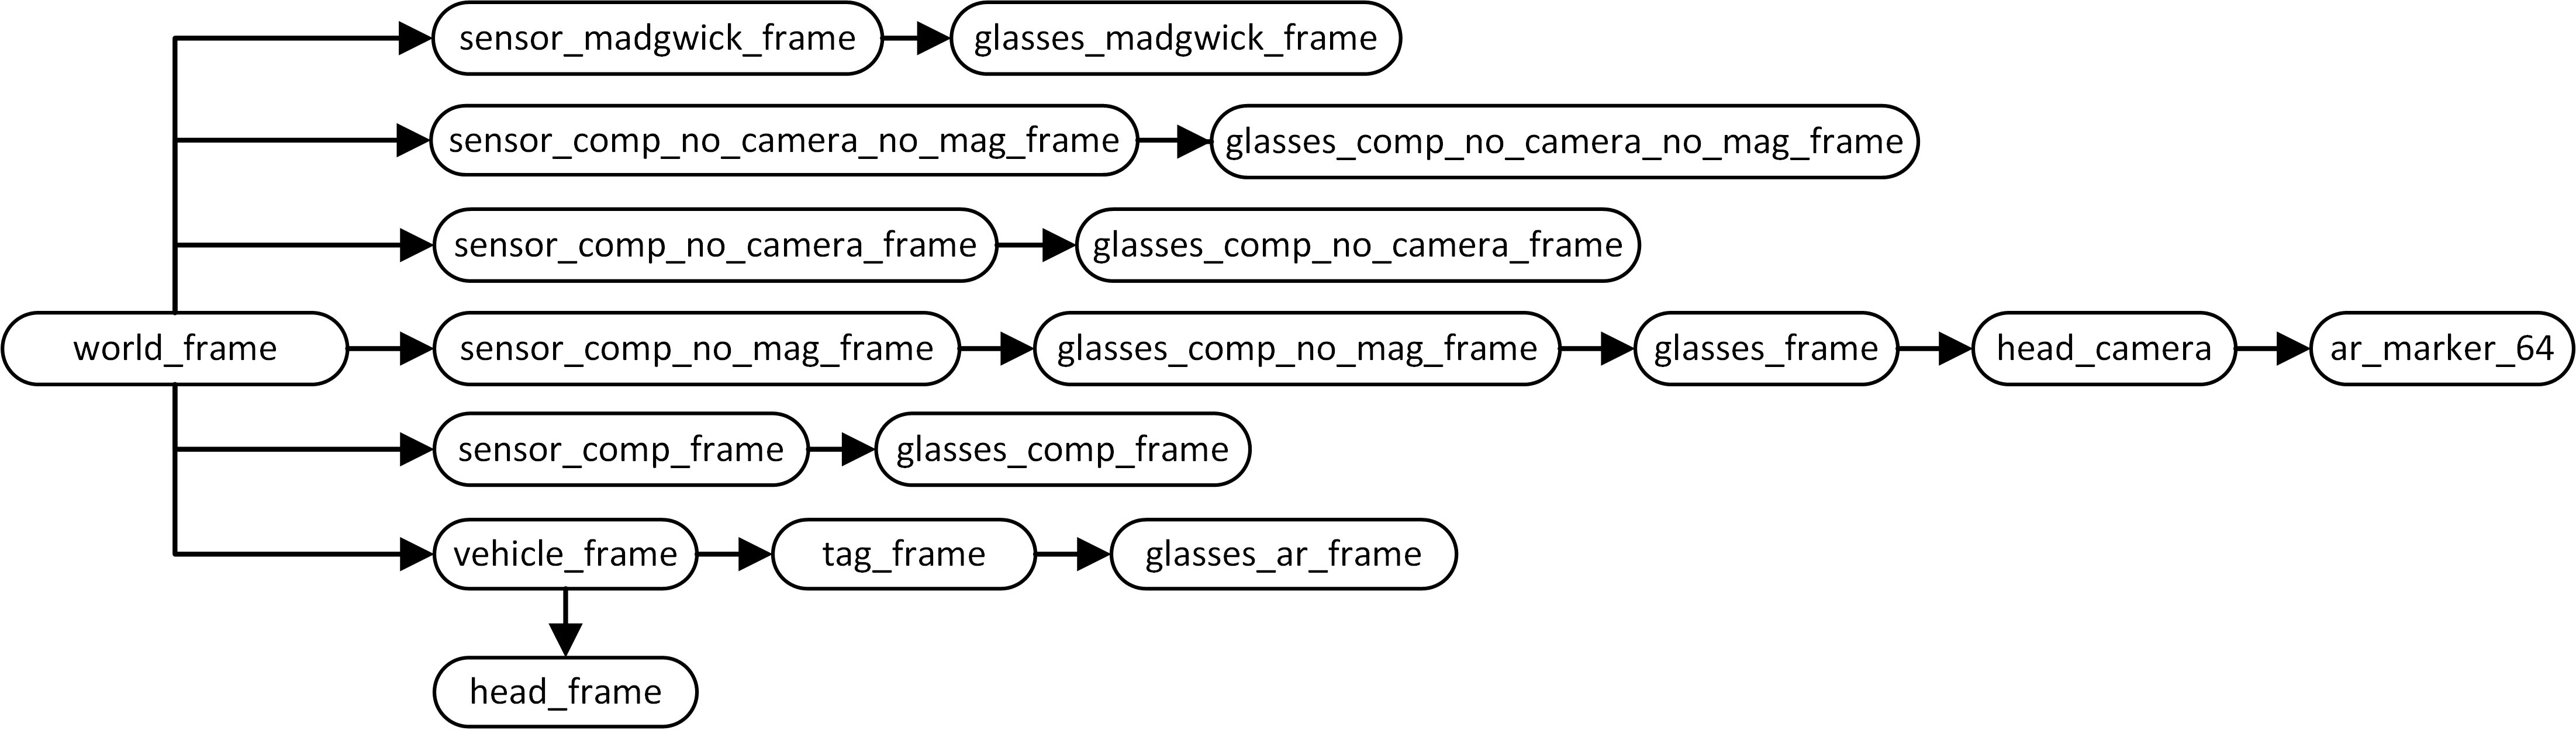
\includegraphics[width=0.98\textwidth]{tf_tree}
  \caption{Koordinaten-Frames}
  \label{fig:tf_tree}
\end{figure*}



\subsection{Ergebnisse}

Die Kopforientierung wird auf Basis verschiedener Sensordaten bestimmt.
Die aus unterschiedlichen Kombinationen der Sensoren berechneten Orientierungen stehen als Ausgabe zur Verfügung:
\begin{itemize}
  \item Marker-Tracking
  \item Gyroskop + Beschleunigungssensor
  \item Gyroskop + Beschleunigungssensor + Magnetometer
  \item Gyroskop + Beschleunigungssensor + Magnetometer + Marker-Tracking
\end{itemize}

Durch Einsatz des \ac{ROS}-Frameworks und durchgängige Verwendung des Transformationsbaums (vgl. Abs. \ref{headtracking_markerfusion_subsubsec}) ist dabei das Referenz-Koordinatensystem frei wählbar.
In der Visualisierung können die gewünschten Berechnungsergebnisse vom Benutzer ausgewählt werden, s. Abb. \ref{fig:kopf_orientierung_rviz}.


Die Applikation konnte erfolgreich im unbewegten \emph{CoCar} getestet werden.
Tests im bewegten Fahrzeug sind noch durchzuführen.


\begin{figure}
  \centering
  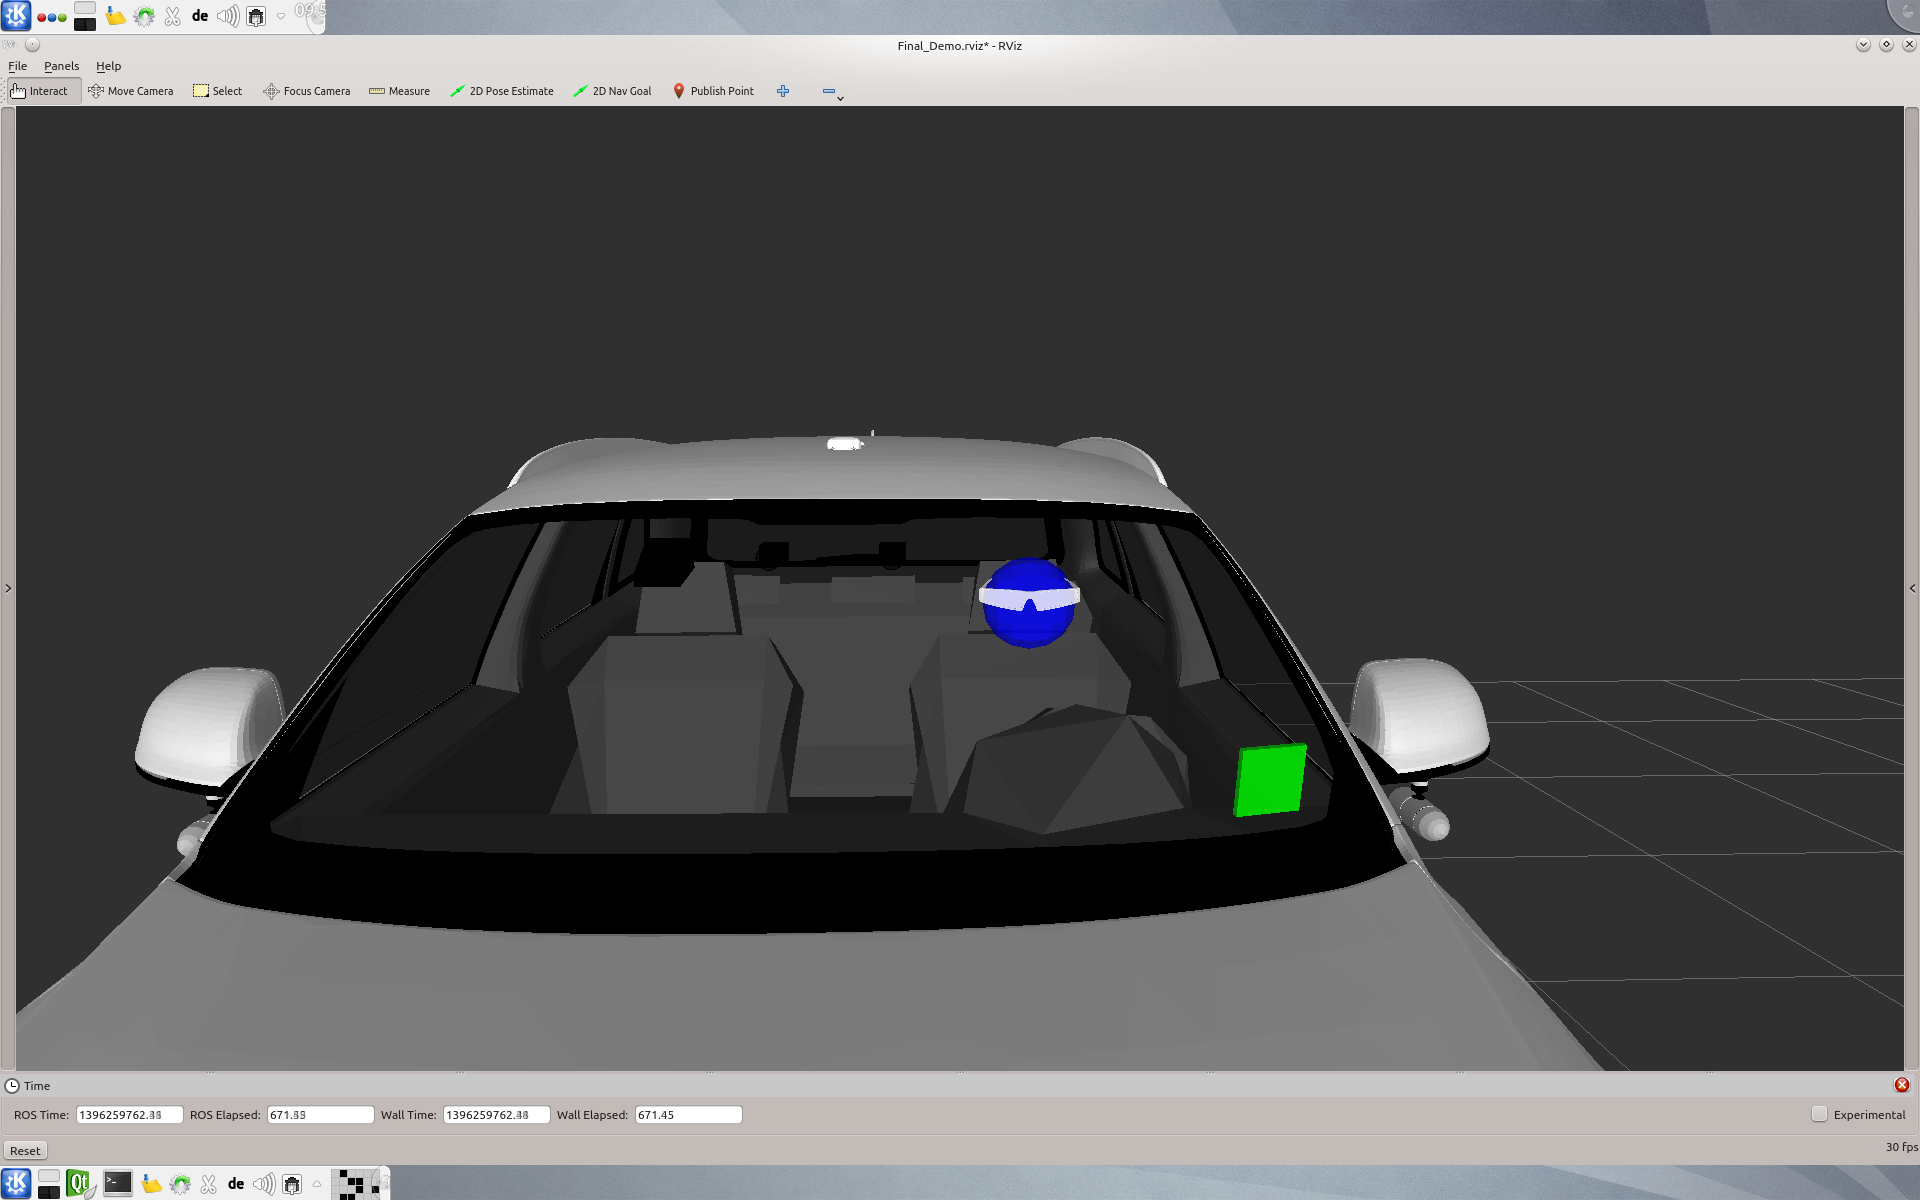
\includegraphics[width=0.4\textwidth]{Frontsicht_Kopf_Brille_RVIZ}
  \caption{Visualisierung der Kopforientierung}
  \label{fig:kopf_orientierung_rviz}
\end{figure}


\subsection{Ausblick}

%\todo[inline]{Irgendwie stimmen ab hier die Absatz-Abstände nicht mehr. Liegt das an der transformations-figure*?} % Ok, stimmen irgendwie doch wieder^^

Für Weiterentwicklungen des Systems bieten sich interessante Bereiche an:

Das System ist derzeit beschränkt auf die Bestimmung der Kopforientierung.
Eine Erweiterung, sodass zusätzlich auch die Position des Kopfes geschätzt wird, ist sicherlich der interessanteste Ansatzpunkt.
Dazu ist eine Integration der Orientierungsdaten über die Zeit nötig.
Da von der in Abs. \ref{headtracking_markertracking_subsubsec} beschriebenen \alvar-Bibliothek auch --bisher nicht verwendete-- Positionsinformationen geliefert werden, kann voraussichtlich die Stützung durch Kameradaten zu großen Teilen unverändert übernommen werden.

Außerdem bietet \alvar \ eine Bundle-Funktionalität, die bisher noch nicht eingesetzt wird.
Damit können im Innenraum des Autos weitere Marker angebracht werden, sodass bei nahezu beliebiger Blickrichtung des Fahrers immer ein Marker im Kamerabild zu erkennen ist.
Die Korrektur der \ac{IMU}-Daten durch Kameradaten wäre damit nicht mehr auf eine Blickrichtung in Fahrtrichtung beschränkt.

Möglich ist auch eine weitere Untersuchung des in Abs. \ref{headtracking_facetracking_subsubsec} beschriebenen Face-Trackings.
Hier ist die Erstellung einer neuen Gesichtsmaske --mit \ac{AR}-Brille-- ein vielversprechender Ansatz.
\todo[inline]{Ist das so? Es gibt doch einige Argumente dagegen. -> siehe Antwort im sourcecode}
% TR: Ich glaube schon, dass es ein Ansatz ist, den man nochmal tiefer angehen könnte. Angeblich funktioniert der bisherige Face-Tracker auch mit normalen Brillen; sprich mit Spiegelung kann er umgehen. Von daher ist der Hauptgrund, dass es bei uns nicht auf Anhieb geklappt hat, wahrscheinlich die falsche Maske. Oder würdest du/ihr das hier raus nehmen?

Ein Ausbau der Hardware-Kompatibilität auf weitere Brillenmodelle wie beispielsweise \emph{Google Glass, Oculus Rift} \oae erscheint ebenfalls interessant.




\section{Kalibrierung der Brille}

Wie kalibriert man eine Durchsichtbrille in einem Auto?

\subsection{Workflow}
    Um eine 3D-Durchsichtbrille so zu kalibrieren, dass auf dieser reale und authentisch wirkende 3D Welten angezeigt werden können, muss präzise kalibriert sein. Wichtig ist dies nur für die prezise Simulation einer AR-Welt. Dies wird wichtig um die Durchsichtbrille für diverse Dinge im UUmfang der kognitiven Automibile zu verwenden. Hierzuu gehören Anwendungen, bei den z.B. Fußgänger SImuliert werden um menschliche Fahrerinteraktionen zu messen und als Lerndaten zu aquireren. Eine weitere Anwendung wäre die SImulation von simulierten Daten des Fahrzeuges für den Fahrer, damit dieser in einer Simulierten Welt beurteilen kann, wie gut das kognitive Automobil sich einer Sitziuation, z.B. dem Einparken verhält. Ebenfalls wird es möglich, mit einer Kalibrierten Brille simulierte neue Bedienelemente eines Autos zu testen und deren Wirkung auf den Fahrer auszuprobieren.

    Hierzu werden die Parameter benötigt, mit denen die Bilder für ein solch akkurates stereoscopic 3D benötigt werden. Zu diesen Parametern zählt die Position der Augen, die Position der Bildschirme in den Brillengläßern und die Öffnungswinkel, mit denen ein einzelnen Individuum durch eine spezifische Brille sehen kann.

    Um diese Parameter zu Bestimmen haben wir uns auf ein interaktives Kalibrierungsverfahren geeinigt, da es wichtig ist, dass die Kalibrierung komfortabel und ohene große Hilfestellung von statten geht, da es für jeden Benutzter nötig ist, die Brille individuell zu kalibrieren. Das Minimum an benötigten Punkten um die Position eines Auges zu bestimmen sind zwei Geraden, also zwei Punkte auf einer Sichtiline je Geraden. Um die Daten präziser zu machen können mehrere Geraden verwendet werden, die dann einen Genaueren Schnittpunkt ermöglichen, es sollen aber immer nur 2 Punkte je Gerade verwendet werden, da das aufeinanderlegen von 3 Punkten in unangenhemen Positionen für den Benutzer während der Kalibrierung endet.

    Der erste Ansstz war es einen Punkt im Auto zu verwenden, der in seiner Position bekannt ist und durhc Bildverarbeitung erkannt werden kann und n Punkte auf der Brille. Hierbei hat sich jedoch herausgestellt, dass der Abstand der einzelnen Schnittlinien in einem sehr kleinen WInkel von statten geht und somit fehleranfällig ist. Der zweite Ansatz verwendet den Bildschirm, der im Auto verbaut ist und die Brillengläser. Hiermit sind beidseitig die Punkte variabel und können somit so gewählt werden, dass sich Messfehler nicht so gravierend auswirken wie im vorherigen Ansatz. Desweiter ist das Verfahren erweiterbar auf eine Onlinebewertung während der Kalibrieung, so dass über ein Algorithmus passende Punkte ausgewählt werden können, um die Kalibrierung zu optimieren.

    Im Ablauf werden nun also Punkte auf dem Brillenglas angezeigt, die der Benutzer per Klick auf die Stelle auf dem Bildschirm markiert, so dass sie für ihn übereinander liegen. Somit konnte ein idealer Kompromiss zwiscen Benutzerfreundlichkeit und der Aquisition von geeigneten Linienpaaren gefunden werden.


\subsection{Bestimmung von Punktepaaren}
\subsubsection{Konzept}
Um nun also Punktepaare für die Kalibrieung aufzeichnen zu können, ist die Grafikausgabe der Software nötig. Hierzu wurden zwei Anwendungen als ROS Nodes implementiert. Die Nodes werden mittels der Frameworks SDL und Qt umgesetzt.
\subsubsection{Anzeige auf der Brille}
Eine Vollbildanzeige mit fester Auflösung der nativen Auflösung der Brillenanzeige wird mittels SDL implementiert. Diese Anwendung erkennt automatisch die Brille als zweiten Bildschirm und wählt diesen für die Anzeige aus. Ansonsten ermöglicht die Anwendung es, einen Punkt an eine per ROS-Paket vorgegebenen Position anzuzeiegn.
Screenshot
\subsubsection{Anzeige auf dem Bildschirm}
Ein Fensteranwendung implementiert mit Qt zeigt die für die Bildverarbeitung nötigen marker (siehe Kapitel??) an und nimmt die Klickpositionen vom Nutzer entgegen. Die ermittelte Clickposition wird als ROS-Paket versendet.
Screenshot!


\subsection{Koordinatentransformation
\subsubsection{\Uumlbersicht}
Die Koordinatentransformationen sind nötig, um aus den Punktepaaren (wie in Kap. ?? beschrieben) , Koordinaten im 3D Weltkoordinatensystem zu erhalten. Nur aus Punkten in einem einheitlichen Koordinatensystem können später korrekte Gerade berechnet werden.
Die Eingaben für das Verfahren erhält die Anwendung aus ROS-Paketen, siehe hierzu in Kapitel ??.
\subsubsection{Weltkoordinatensystem}
Das Weltkoordinatensystem für die Transformation hat seinen Ursprung in der Camera, gerichtet in Scihtrichtung mit der Knvention angelehnt an Kamerasysteme: x nach rechts  ,y nach unten, z nach vorne.
\subsubsection{Transformation für Brillenpunkte}
Das ausgewählte Koordinatensystem macht es einfach die Transformation von einem Brillenpixel in das Weltkoordnitensystem abzubilden. Es handelt sich um eine statische Transformation, da die Camera fest mit der Brille verschraubt ist. Die Herausforderung besteht darin, den virtuellen Bildschirm der Brille abzubilden. In den einzelnen Brillengläsern befindet sich Optik (Lines und ein Spiegel), mit denen dem Brillenträger ein großer Bildschirm Simuliert wird. Da es für uns jedoch nicht möglich war, festzustellen, ob für jeden Brillenträger die Anzeige gleich war, haben wir folgenden Verfahren angewendet: Wir haben den virtuellen Bildschirm, projeziert per strahlensatz, auf einen weiteren virtuellen Bildschirm genau im Mittelpunkt der Brille festgelegt. Dieser Bildschirm ist unabhängig vom Benutzer, da zu Vermessung dieses Bildschirmes der Abstand zum virtuellen Bildschirm keine Rolle spielt.
Die Wahl des virtuellen Bildschirms genau in der Brillenmitte hat ebenfalls den Vorteil, dass die gewonnenen Daten später auch für die Berechnung des Öffnungswinkels verwendet werden können, da diese identisch mit den physikalischen Brillengläsern sind.
Die Position des Bildschrimes wurd aus empirischen Ergebnissen gewonnen. Hierzu haben wir die Brille wagerecht zu einer Wand festgeschraubt und Punktepaare zu einem von Hand vermessenen Auge aufgenommen. Hierzu haben wir Punktekoordinaten auf dem Bildschirm zu konstanten Punkten auf der waagerecht zur Brille montierten Referenzwand (mit Punkten) vermessen. Die Brille wurde in die für den jeweiligen Probanden korrekte Position gebracht, so dass es genau für einen Öffnungswinkel die Referenzwand füllend im Bild sehen kann. Anschließend wird der Abstand zur Wand vermessen. Aus dem Abstand zur Wand und den Vermessenen Punkten auf der Wand, konnte mit Hilfe der gemessenen Pixel auf der Brille, die größe eines Pixel auf unserem virtuellen Bildschirm innerhalb der Brille erechnet werden. Der Abstand auf dem referenzbildschirm war für jeden Probanden gleich, die angeklickte Position war ebenfalls gleich, jedoch der Abstand zur Wand leicht verschieden, da verschiedene Probanden einen leicht Abweichenden Sichtöffnungswinkel hatten, da die Augen je nach physiologischen Eigenschaften verschieden weit hinter der Brille sich befinden. Hierdurch war es uns möglich eine Fehlerrechnung über alle Daten durchzuführen, da wir 15 Punkteppare hatten. Hierdurch kamen wir zu relativ genauen Ergebnissen des Brillenbildschirms:
    
    Statisch ermittelte Werte:
    Pixelgröße (links und rechts):      2.5219887302047E-02 cm/px 
    Größe des virtuellen Bildschirms (links und rechts):      1
    Position des Bildschirms (links):
    Position des Bildschirms (rechts):
        
Durch diese Ausmessungen konnte die  Transformation eines Koordinatenpunktes u,v in Weltkoordinaten auf zwei einfache Transformationen vereinfacht werden

    1. Statische Transformation: Translation vom Oberen linken virtuellen Bildschirmpixel zum Ursprung

    2. Dynamische Transformation: Translation um u,v Pixel nach obiger Vermessung umgerechnet in Meter

In der Implementierung wurde noch folgende Vereinfachung festgestellt: Da die virtuellen bildschirme immer eine parallele Ebene zur x,y-Achsen-Ebene aufstellen, kann die transformation durch eine einfache Addition durchgeführt werden

    Listing einfügen.

\subsubsection{Transformationen für Bildschirmpunkte}
Die Transformation von einem Bildschirmpixel in das Weltkoordinatensystem stellt andere Herausforderungen. Der Bildschirm kann als eine physikalische Gröse angesehen werden und vermessen werden. Es liegen konstante DPI-Werte vor, es kann also ebenfalls eine statische Transformation von einem Referenzpunkt auf dem Bildschirm zum angeziegten Punkt geschehen. Hierzu ist lediglich eine Transformation nötig, die die DPI-Werte des Bildschirms berücksichtigt und durchführt. Der Referenzpunkt des Bildschirms haben wir innerhalb unserer Anwendung (sihe Kapitel ??) gewählt, da dieser somit invariant gegen verschiebungen bleibt. Bei diesem Vorgehen besteht jedoch die größte Herausforderung darin, dass die Position des Bildschirmes benötigt wird. Heirzu wird die Camera mit Bildverarbeitung eingesetzt. Der erste Ansatz war es, openCV mit einem Schachbrett zur Erkennung zu verwenden. Da sich während der Implementierung herausgestellt hat, dass einiger Code, der beim Einsatz von openCV nötig ist, durch die Bibiolothek ALVAR, die sich ebenfalls noch wesentlich einfacher in ROS integrieren lässt abnimmt, wurde die Strategie geändert. Drei ALVAR Marker werden nun mittels der Webcam erkannt und zur Entfernungsbestimmung vermittelt. Hiermit sind nun beide Transformatione auch für die Berechnung der Position vorhanden. Dieser Ansatz bietet den Nachteil, dass ALVAR eine gewisse ungenauigkeit und eine gewisse Verzögerung mit sich bringt, wodurch die Benutzbarkeit erschwert wird. Ein längerfristiges Ziel sollte es also sein, die Integration des Headtrackingalgorithmuses auch in die Kalibrieung einzufügen.
    Statisch ermittelte Werte:
    Pixelgröße:
    Größe eines Markern in Pixeln/CM:
Das Konkrete Vorgehen beschreibt sich bezüglich der Transformation folgendermaßen:

    1. Dynamische Transformation:  Translation  um u,v der auf der Fensterfläche angeklickt wurde auf den Referenzpunkt der Anwendung (konkret, dem Mittelpunkt des obigen linken Markers) 

    2. Dynamische Transformation: Translation um die von ALVAR bestimmte entfernung

Um auf den Referenzpunkt zu gelangen, gibt es eine triviale Addtion, um den statischen Offset der Anzeigelemente und der centrierten ALVAR position zu kompensieren. Um nun die Translation um einen u,v Pixel zu realisiren, wird eine Ebene durch die drei marker gelegt und daruf die Verschiebung durchgeführt. Im Anschlass kann die Rücktransformation zum Koordinatenursprung geschehen.

    Listing einfügen



\subsection{Stereoskopisches 3D}

\subsubsection{Allgemeine Information}
Es existieren mehrere Gründe des menschliches Raumwahrnehmung.
Menschen sehen die Objekte dreidimensional wegen der Linearperspektive, relativer Größe zur anderen Objekte, Verdeckung der Objekten und wegen stereoskopisches Sehen. 
Stereoskopisches Sehen vermittelt durch die beidäugige Betrachtung von Objekten und Gegenständen eine echte, messbare Tiefenwahrnehmung und räumliche Wirkung des Außenraums. 
Das passiert mit der Hilfe beider unseren Augen.
Jede Auge bekommt ein eigenes Bild und sendet das ins Gehirn. 
Dort werden diese beide Bilder zu eine einzige zusammengefasst.
Genauere Beschreibung ist im Abb. \ref{fig:3D} zu finden.

\begin{figure}[h]
   \centering
   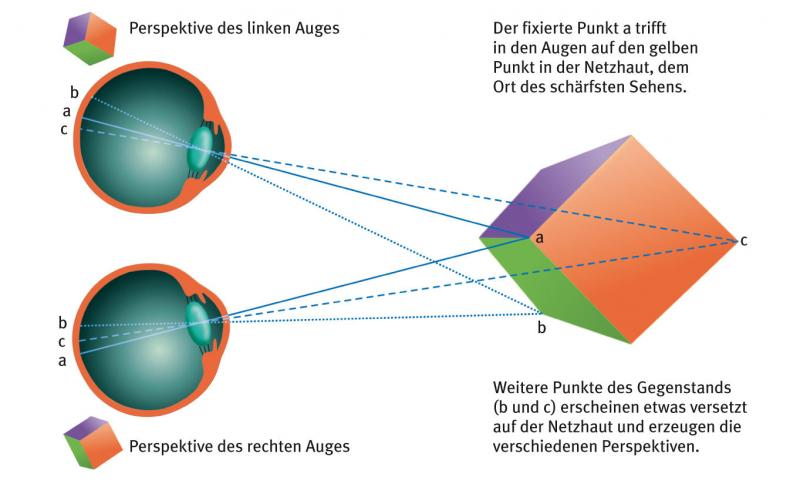
\includegraphics[width=0.45\textwidth]{3D-bild}
   \caption{steteoskopisches Sehen}
   \label{fig:3D}
\end{figure}

Die Bilder des linken und rechten Auges sich an manchen Stellen unterscheiden und menschliches Gehirn kann aus dieser Unterschiede die Positionen, Formen und Großen der Objekte extrahieren.

Damit ein Bild dreidimensional aussieht, ist meistens genug mit ungefähren Werten zu arbeiten.
Man nimmt zwei unterschiedliche Bilder, die anhand der mittlere Werte ausgerechnet werden, und zeigt jeder Auge eine davon. 
Damit bekommt man ein 3D-Bild. 
Für manche Anwendungen (wie 3D-Filme, oder sterioskopische Bilder) ist schon genug,  dass ein Bild als 3D interpretiert wird. 
Für uns aber nicht, da mit so eine Realisation unterschiedliche Menschen sehen dasselbe Bild unterschiedlich.
Alle Menschen werden diese Bilder als 3D interpretieren, aber die Position und Größe der gesehenen Objekte kann sich stark unterscheiden.
Für die Anwendungen, wie Testen des autonomes Fahrens des Fahrzeugs, sind aber diese Werte entscheidend.
Es ist sehr wichtig, ob ein anderes Fahrzeug schon getroffen ist, oder nicht.
Um die benötigte Genauigkeit zu realisieren, sind gemittelte Werte nicht genug.
Eine individuelle Kalibrierung der Brille soll diese Genauigkeit ermöglichen.

\subsubsection{Geometrische Beschreibung der Kalibrierung}
Dieses Kapitel beschreibt wofür die Kalibrierung durchgeführt wird und welche Daten dafür benötigt werden.
Die gegebene Daten sind im Abb. \ref{fig:geom} dargestellt. 

\begin{figure}[h]
   \centering
   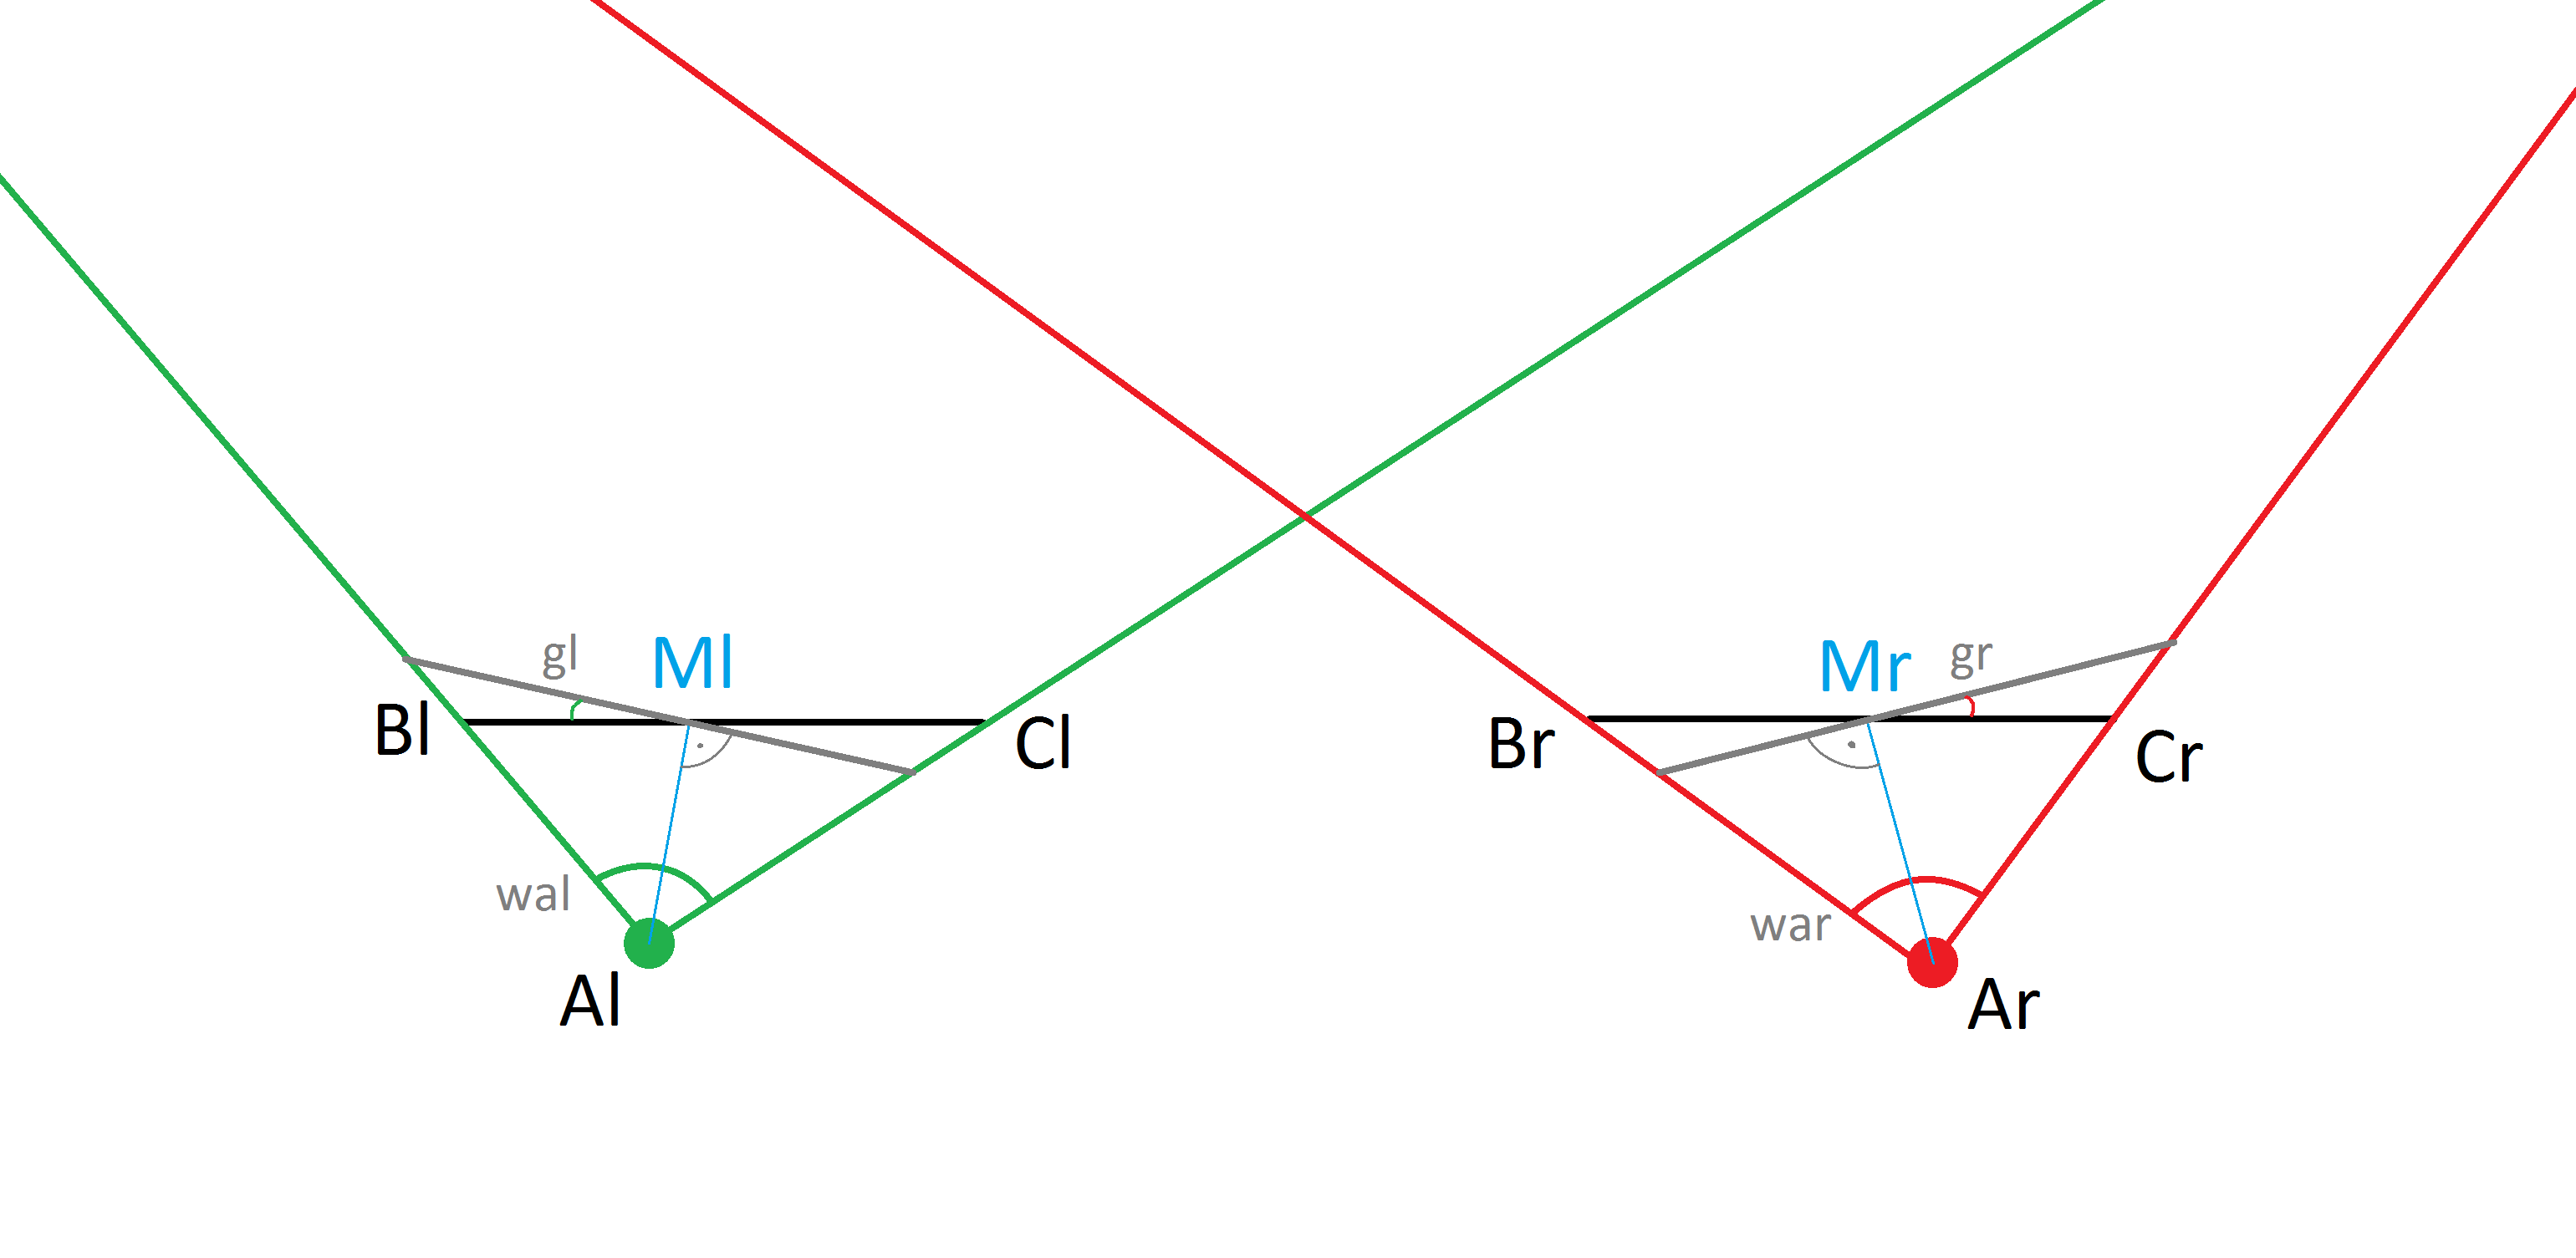
\includegraphics[width=0.45\textwidth]{kalibr-geometrie}
   \caption{Geometrische Beschreibung der Kalibrierung}
   \label{fig:geom}
\end{figure}

Punkte Bl, Cl bzw. Br, Cr sind die Endpunkte des linkes bzw. rechtes Bildschirms der Brille.
Die Punkte Al (grün) bzw. Ar (rot) beschreiben die Positionen der Augen.
wal bzw. war sind die Sehwinkel des Benutzers durch welche die Bildschirme und dort dargestellte Objekte gesehen werden. 
Blaue Linien ml und mr sind Winkelhalbierenden.

Für die Anzeige der Bilder auf der Brillenbildschirme, werden Augen als Kameras interpretiert und damit werden benötigte Bilder erstellt.
Dementsprechend sind die Winkeln wal und war die Öffnungswinkel dieser Kameras.
Wie auf dieser Abb. ref{fig:geom} gut zu sehen ist, müssen die Augepositionen nicht unbedingt in der mitte des Bildschirms liegen.
In meisten Anwendungen, die Kameras simulieren, ist aber vorausgesetzt, dass die Kameras in der Mitte sind.
Das ist das selbe, wie Winkelhalbierende der Öffnungswinkel senkrecht zur Bildschirm ist.
Wir nehmen an, dass dafür benötigte Drehwinkel gl bzw. gr spielt keine entscheidende Rolle in der Bildanzeige.
Mit dieser Annahme rechnen wir die Winkeln gl und gr aus  um die Virtuelle Bildschirme theoretisch zu drehen.
Das wird benötigt um passende Daten für die Benutzung anderer Anwendungen zu bekommen.





%\section{Zusammenfassung}
Alles was ans Ende gehört.
\subsection{Ausblick}
\subsection{Fazit}

% Can use something like this to put references on a page
% by themselves when using endfloat and the captionsoff option.
\ifCLASSOPTIONcaptionsoff
  \newpage
\fi



% trigger a \newpage just before the given reference
% number - used to balance the columns on the last page
% adjust value as needed - may need to be readjusted if
% the document is modified later
%\IEEEtriggeratref{8}
% The "triggered" command can be changed if desired:
%\IEEEtriggercmd{\enlargethispage{-5in}}



% references section

% can use a bibliography generated by BibTeX as a .bbl file
% BibTeX documentation can be easily obtained at:
% http://www.ctan.org/tex-archive/biblio/bibtex/contrib/doc/
% The IEEEtran BibTeX style support page is at:
% http://www.michaelshell.org/tex/ieeetran/bibtex/
\bibliographystyle{IEEEtran}
% argument is your BibTeX string definitions and bibliography database(s)
\bibliography{bibliography/ausarbeitung}
%
% <OR> manually copy in the resultant .bbl file
% set second argument of \begin to the number of references
% (used to reserve space for the reference number labels box)
%\begin{thebibliography}{1}
%
%\bibitem{IEEEhowto:kopka}
%H.~Kopka and P.~W. Daly, \emph{A Guide to {\LaTeX}}, 3rd~ed.\hskip 1em plus
%  0.5em minus 0.4em\relax Harlow, England: Addison-Wesley, 1999.
%  
%\end{thebibliography}

% that's all folks
\listoftodos
\end{document}
